\documentclass{article}
%% \documentclass[dvipdfmx,a4paper]{article}


%%% macros
%%\input{narrowermargin} %% lncs contents with narrower margins
%%% begin: papersize with narrower margins
%% \usepackage[papersize={50mm,50mm}]{geometry}
%%% narrowmargin.tex
%%% begin: papersize with narrower margins
\usepackage{calc}
\newlength{\marginwidth} %% 
\newlength{\contentswidth} %% lncs
\newlength{\contentsheight} %% lncs
\newlength{\mypaperwidth} %% paper
\newlength{\mypaperheight} %% paper
\setlength{\marginwidth}{20mm} %% 
\setlength{\contentswidth}{145mm} %% lncs
\setlength{\contentsheight}{225mm} %% lncs
\setlength{\mypaperwidth}{\contentswidth+\marginwidth} %% paper
\setlength{\mypaperheight}{\contentsheight+\marginwidth} %% paper
\usepackage[papersize={\mypaperwidth,\mypaperheight},margin=\marginwidth]{geometry} 
%%% end: papersize 
%%% EOF

%% \input{myarith}
%%% end: papersize
\usepackage{amsmath,amssymb}
\usepackage{amsthm} %%proof environment
%%% auto labeling
\usepackage{mathtools}
\mathtoolsset{showonlyrefs=true}
%%% end: auto labeling
\usepackage{enumerate}
\usepackage{booktabs}
\usepackage{graphicx}
\graphicspath{
  {latex/fig/}
  {fig/}
  {fig/new/}
}%%画像のパス.末尾は'/'で終わること
%%%% algo
\usepackage[ruled,vlined,linesnumbered]{algorithm2e}
%%% setting: algorithm2e %%%%%%%%%%%%%%%%%%%%%%%%%%%%%%%%
\newcommand{\algoopts}{%
%%% RULES
%boxed,%good
%boxruled,%
%algoruled,%good
ruled,%
%tworuled,%
%%% CODE TYPESETTING
%% hangingcomment,%
%% opthanginginout,%
%% noalgohanging,%obsolute 
%%% BLOCKS DISPLAY
%noline,%
vlined,%L-tyle
%lined,%I-style
%%%
linesnumbered%
}
%%\usepackage[\algoopts]{algorithm2e} 
\usepackage[ruled,vlined,linesnumbered]{algorithm2e} 

\makeatletter
\renewcommand{\@algocf@capt@plain}{above}% formerly {bottom}
\makeatother
%%% algorithm2e
\newcommand{\comblk}[1]{\hfill$\rhd$\ \textit{#1}}
\newcommand{\Commentblock}[1]{\comblk{#1}}
\newcommand{\Commentblockl}[1]{\kern0.5em$\rhd$\ \textit{#1}\ $\lhd$}
\newcommand{\CM}[1]{\comblk{#1}}
%% \SetArgSty{textrm}%arguments for e.g., if, else, while etc. 
%% \SetCommentSty{textit}%arguments for comments
\SetKwComment{Comment}{$\rhd$}{} 
\SetKwInput{KwInput}{Input}
\SetKwInput{KwOutput}{Output}
\SetKwInput{KwNotes}{Notes}
%%%
\SetKwInput{KwPreproc}{Preprocess}
\SetKwInput{KwRuntime}{Runtime}
\SetKwInput{KwGiven}{Given}
\SetKwInput{KwGlobal}{Global}
\SetKwInput{KwWork}{Working}
\SetKwInput{KwMethod}{Method}
\SetKwInput{KwPrecond}{Pre-condition}
\SetKwInput{KwPostcond}{Post-condition}
\SetArgSty{textrm}%arguments for e.g., if, else, while etc. 
\SetCommentSty{textit}%arguments for comments
\newcommand{\iIf}[2]{\textbf{if} {#1} \textbf{then}\hspace{0.125em}{\relax #2}}
\newcommand{\iElseIf}[2]{\textbf{else if} {#1} \textbf{then}\hspace{0.125em}{\relax #2}}
\newcommand{\iElse}[1]{\textbf{else} {\relax #1}}
\newcommand{\iFor}[2]{\textbf{for} {#1} \textbf{do}\hspace{0.125em}{\relax #2}}



%%%
%% \usepackage{natbib}
%\setcitestyle{numbers,super}
%%%
\usepackage{tikz}
\usetikzlibrary{calc}
%\usetikzlibrary{intersections,calc,arrows.meta}

%%% macro private
%%% config.tex

%%======================================
\usepackage{graphicx}
%% \usepackage{amsmath,amssymb}
%% \usepackage{mathtools}
%% \mathtoolsset{showonlyrefs=false} %% 参照している式参照のみ表示
%% \mathtoolsset{showonlyrefs=true} %% 参照している式参照のみ表示
%% \usepackage{cite}
\usepackage{caption}    %%for subfigure
\usepackage[skip=0.5ex]{subcaption} %%for subfigure
\captionsetup{aboveskip=0.0\baselineskip}
\captionsetup{belowskip=0.0\baselineskip}
%%%
%%\usepackage{titlesec}
%% \titlespacing*{\section}{0pt}{5.5ex plus 1ex minus .2ex}{4.3ex plus .2ex}
%% \titlespacing*{\subsection}{0pt}{5.5ex plus 1ex minus .2ex}{4.3ex plus .2ex}

%%% table
%% \usepackage{multirow}
\usepackage{booktabs}
\usepackage{array}

% private macros by others 
\usepackage{url}
\usepackage{bm}
\usepackage{textcomp}%%for cent
%\usepackage[margin=1.75in]{geometry}
%\usepackage[margin=1.0in]{geometry}
%% \usepackage{subfig}
%% \usepackage{natbib}

%%% private %%%%%%%%%%%%%%%%%%%%%%%%%%%%%%%%%%%%%

%% private macros by arim@ist
%%% jsvmac.tex
%%% macros from a subset of jsv1.sty 

%%% from jsv1.sty

% Write multichar identifier names using \id in either mathmode or text;
% For ex, $\id{high}(x)$ is an expression using the \id{high} function.
% Use ``\ '' if a space is desired, as in math mode.
\def\id#1{\ensuremath{\mathit{#1}}}
\let\idit=\id
\def\idbf#1{\ensuremath{\mathbf{#1}}}
\def\idrm#1{\ensuremath{\mathrm{#1}}}
\def\idtt#1{\ensuremath{\mathtt{#1}}}
\def\idsf#1{\ensuremath{\mathsf{#1}}}
\def\idcal#1{\ensuremath{\mathcal{#1}}}  % Use with capital letter args only
\def\idsc#1{\ensuremath{\textsc{#1}}} % added by arim

%%% end jsv1.sty

%%% EOF

%%\input{arimmacro} %%privatemacro


%%%%%%%%%%%%%%%%%%%%%%%%%%%%%%%%%%%%%%%%
%%xsavebox
\usepackage{xsavebox}

%%%%%%%%%%%%%%%%%%%%%%%%%%%%%%%%%%%%%%%%%
%%% above and below float figure table
\setlength\intextsep{0.5\baselineskip}
\setlength\abovecaptionskip{0.0\baselineskip}
\setlength\belowcaptionskip{0.5\baselineskip}
%% \setlength\intextsep{18pt}

%%%%%%%%%%%%%%%%%%
%% latex native savebox and lrbox
\newenvironment{savethm}[1]{\begin{lrbox}{#1}\begin{minipage}[t]{1.0\textwidth}}{\end{minipage}\end{lrbox}}

\newcommand{\putthm}[1]{
%% \smallskip
\noindent 
\usebox{#1}
\medskip}

%%sample
%% \newsavebox{\thmbox}
%% \begin{lrbox}{\thmbox}
%% \begin{minipage}[t]{1.0\textwidth}
%% \begin{theorem}\label{thm:algbwt:main}
%% ....
%% \end{theorem}
%% \end{minipage}
%% \end{lrbox}


%% \putthm{\thmbox}


%%%%%%%%%%%%%%%%%%




%%%%%%%%%%%%%%%%%%%%%%%%%%%%%%%%%%%%%%%%
%%comment out a paragraph
\newsavebox{\cmbox}
\newenvironment{commbox}{
  \begin{lrbox}{\cmbox}
    \begin{minipage}{.9\textwidth}
}{\end{minipage}
  \end{lrbox}
  %\framebox{\usebox{\cmbox}}
}


%%%%%%%%%%%%%%%%%%%%%%%%%%%%%%%%%%%%%%%%
% %%% empty environment 
% \newenvironment{myempty}{\begin{commbox}}{\end{commbox}}
% %%% proof environment 
% \newenvironment{myproof}{\begin{proof}}{\end{proof}} %default
% \newenvironment{myfullproof}{\begin{proof}}{\end{proof}} %default
% \newenvironment{myfullproofempty}{\begin{myempty}}{\end{myempty}} %default

%% replace an enviroment #1 with #2
\newcommand{\myenvironmentreplace}[2]{\renewenvironment{#1}{\begin{#2}}{\end{#2}}}

%% claim %%
\newenvironment{myclaim}[1][]{\bgroup\parskip=0mm\par (\textit{Claim{#1}})}{(\textit{End of Claim})\par\egroup}  
\newenvironment{proofofclaim}{\bgroup\parindent=1em\parskip=0mm\par (\textit{Proof for the claim})}{(\textit{End of the proof for the claim})\par\egroup}  
\newenvironment{proofofclaimempty}{\begin{myempty}}{\end{myempty}}

%% \newenvironment{proofofclaim}{\bgroup\parskip=0mm\par (Proof for the claim)}{(End of the proof for the claim)\par\egroup}  


%%%%%%%%%%%%%%%%%%%%%%%%%%%%%%%%%%%%%%%%

% %% switch catcode of '&' between 4 and 9
% \newenvironment{inalign}{\begin{math}\catcode`&=9}{\catcode`&=4\end{math}}

%%%%%%%%%%%%%%%%%%%%%%%%%%%%%%%%%%%%%%%%

% lipics predefined

%% send a proof to the appendix
\newtheorem{definition}{Definition}
\newtheorem{theorem}{Theorem}
\newtheorem{lemma}[theorem]{Lemma}
\newtheorem{proposition}{Proposition}
\newtheorem{corollary}[theorem]{Corollary}
\newtheorem{remark}{Remark}
\newtheorem{fact}{Fact}
\newtheorem{condition}{Condition}

% \newtheorem{example}[example]{Example}[section]
% \newtheorem{conjecture}{Conjecture}
% %% dammy
%%%%%%%%%%%%%%%%%%%%%%%%%%%%%%%%%%%%%%%%

%%% cleveref
\usepackage{cleveref}
\crefname{section}{Sec.}{Sections}
\crefname{chapter}{Chapter}{Chapters}
%%
\crefname{algorithm}{Algorithm}{Algorithms}
\crefname{table}{Table}{Tables}
\crefname{figure}{Fig.}{Figures}
%% 
\crefname{definition}{Definition}{Definitions}
\crefname{lemma}{Lemma}{Lemmas}
\crefname{proposition}{Prop.}{Propositions}
\crefname{theorem}{Theorem}{Theorems}
\crefname{remark}{Remark}{Remarks}
\crefname{fact}{Fact}{Facts}
\crefname{condition}{Condition}{Conditions}
\crefname{problem}{Problem}{Problems}
\crefname{observation}{Observation}{Observations}
%% \crefname{lemma}{Lemma}{Lemmas}
\crefname{equation}{Eq.}{Equations}
%%% fix of a bug in Algorithm
\newcommand{\aref}[1]{Algorithm\kern0.25em\ref{#1}} 
%%%%%%

% %% send a proof to the appendix
\usepackage{apxproof}
% \newtheoremrep{definition}{Definition}[section]
\newtheoremrep{lemma}[theorem]{Lemma}[section]
\newtheoremrep{proposition}[proposition]{Proposition}[section]
\newtheoremrep{theorem}[theorem]{Theorem}[section]
\newtheoremrep{corollary}[theorem]{Corollary}[section]
% \newtheoremrep{remark}[theorem]{Remark}

%% \newtheoremrep{example}[example]{Example}[section]
%% \newtheoremrep{conjecture}{Conjecture}
%% %% dammy
%% \newcommand{\resetrep}{}
%% rest 
%% \newcommand{\resetreptext}{{\rm\textsf{in draft}}}
%% \newcommand{\getfollow}[1][{}]{{\rm\textsf{(*{#1})}}\ }

%% \newcommand{\resetrep}{%% resetting all rep-style environments
%% %% \renewenvironment{lemmarep}{\begin{lemma}\getfollow}{\end{lemma}}
%% \renewenvironment{lemmarep}{\begin{lemma}\getfollow}{\end{lemma}}
%% \renewenvironment{propositionrep}{\begin{proposition}\getfollow}{\end{proposition}}
%% \renewenvironment{theorem}{\begin{theorem}\getfollow}{\end{theorem}}
%% \renewenvironment{corollaryrep}{\begin{corollary}\getfollow}{\end{corollary}}
%% \renewenvironment{examplerep}{\begin{example}\getfollow}{\end{example}}
%% \renewenvironment{remarkrep}{\begin{remark}\getfollow}{\end{remark}}
%% \renewenvironment{conjecturerep}{\begin{conjecture}\getfollow}{\end{conjecture}}
%% \renewenvironment{toappendix}{}{}
%% }

%%%%% 
\newenvironment{statement}[1]{\begin{trivlist}\item[]$\blacktriangleright\:$\textbf{#1}\ }{\end{trivlist}}
\newenvironment{notoappendix}{}{} %% the empty version of toappendix

%%%%%%%%%%%%%%%%%%%%%%%%%%%%%%%%%%%%%%%%%
%% enumitem: smart enumerate and itemize
%% the vspace above list = \topsep + \parskip + \partopsep
%% the vspace between items = \itemsep + \Parsep 
%% the vspace between paragraphs = \Parsep 
\usepackage[inline,shortlabels]{enumitem} %enumerate
\setlist{noitemsep}
\setlist{%
topsep = 0.25\baselineskip,
parsep = 0.125\baselineskip
}%exp
\setlist[enumerate]{ labelsep=.25pc, leftmargin=1.5pc } 
%% \setlist[enumerate]{ labelsep=.25pc, leftmargin=1.5pc } 
\setlist[enumerate,1]{ label= (\arabic*), ref=\arabic*}
\setlist[enumerate,2]{ label= (\roman*),ref  = \roman*}
\setlist[enumerate,3]{ label= (\alph*), ref  = (\alph*)}
%\setlist[itemize]{ leftmargin=1.5pc }
\setlist[description]{ font=\sffamily\bfseries }
%% end macros
%%% switch
%% \newenvironment{myenumerate}{\begin{enumerate}}{\end{enumerate}}
\newenvironment{myenumerate}{\begin{enumerate*}}{\end{enumerate*}}
%% end macros

%%

%% %% 目次のハイパーリンク: 印刷時は念の為コメントアウト(本来出ない)
%% \usepackage[%
%% %dvipdfmx,%
%% colorlinks=true,%
%% linkcolor=blue,%
%% anchorcolor=black,%
%% citecolor=blue,%
%% urlcolor=blue%
%% ]{hyperref} %注意:パッケージの最後に読み込むこと

%%%%

%% EOF

%%% 数式モードで使う表記
\newcommand{\set}[1]{\{#1\}}
\newcommand{\iffdef}{\stackrel{\idrm{def}}{\iff}}
\renewcommand{\mod}{\idrm{mod}}
\newcommand{\Key}[1]{\Statex\hspace{-1.2\leftmargin}  \textbf{#1}\hspace{.25em}}
\newcommand{\Proc}[1]{\Key{Procedure}{#1}}
%\newcommand{\Proc}[1]{\Statex\hspace{-1.2\leftmargin}  \textbf{Procedure}\hspace{.25em}{#1}}
\newcommand{\ename}[2]{\textbf{#1} (\textit{#2})}
\newcommand{\itl}[1]{\textit{#1}}
\newcommand{\sig}[1]{\mathcal{#1}}

%%% 数式モードで文字が開く問題を解消する機能

\def\id#1{\ensuremath{\mathit{#1}}}
\let\idit=\id
\def\idbf#1{\ensuremath{\mathbf{#1}}}
\def\idrm#1{\ensuremath{\mathrm{#1}}}
\def\idtt#1{\ensuremath{\mathtt{#1}}}
\def\idsf#1{\ensuremath{\mathsf{#1}}}
\def\idcal#1{\ensuremath{\mathcal{#1}}} 

%%% 参照の便利版
\usepackage{cleveref}
\crefname{algorithm}{アルゴリズム}{Algorithms}
\crefname{table}{表}{Tables}
\crefname{figure}{図}{Figures}
\crefname{section}{節}{Sections}
\crefname{chapter}{章}{Chapters}
\crefname{problem}{問題}{Problems}
\crefname{definition}{定義}{Definitions}
\crefname{lemma}{補題}{Lemmas}
\crefname{fact}{事実}{Facts}
\crefname{property}{性質}{Properties}
\crefname{proposition}{命題}{Propositions}
\crefname{thmeorem}{定理}{Theorems}
\crefname{cor}{系}{Corollaries}
\crefname{footnote}{脚注}{Footnotes}
%%% notation.tex


%%%% new atoc 
\newcommand{\Sub}{\idsf{Sub}}
%% \newcommand{\Suf}{\idsf{Suf}}
%% \newcommand{\Pref}{\idsf{Pref}}
\newcommand{\LPF}{\idrm{LPF}}

\newcommand{\SA}{\idrm{SA}}
\newcommand{\ISA}{\idrm{ISA}}
\newcommand{\LCP}{\idrm{LCP}}
\newcommand{\BWT}{\idrm{BWT}}

%%%%

%%% algo
\newcommand{\RecLPT}{\textsf{RecLPT}}  %% TDSA
\newcommand{\RecCDAWG}{\textsf{RecCDAWG}}  %% TDSA
\newcommand{\SkipAndCount}{\textsf{SkipAndCount}}  %% TDSA
\newcommand{\FindNonEquivLocus}{\textsf{FindLongestPrefixPath}}  %% TDSA

\newcommand{\MREnum}{\textsf{Enum}}  %% TDSA
\newcommand{\GenChildren}[1][{\LCP}]{\textsf{GenChildren}_{#1}}  
\newcommand{\ColoredRange}[1][{\BWT,RMQ}]{\textsf{ColoredRange}_{#1}}  
\newcommand{\append}{\op{append}}

\newcommand{\LChar}[1][S]{\idrm{LChar}_{#1}}
\newcommand{\RChar}[1][S]{\idrm{RChar}_{#1}}
\newcommand{\getfactor}[1][{\SA, S}]{\op{Fact}_{#1}} 
\newcommand{\isLeftBranching}[1][{\SA, \ISA, S}]{\proc{isLeftBranching}_{#1}}\newcommand{\RREP}{\mathcal{RP}}  %% TDSA

%%%
%% \newcommand{\rk}[1]{^{(#1)}} %%alias 
\newcommand{\idx}[3]{_{#1=#2}^{#3}} %%alias
%% \newcommand{\btw}[3]{{#2}\le {#1}\le {#3}} %%alias
%% \newcommand{\Suf}{\idrm{Suf}}
%% \newcommand{\Fac}{\idrm{Fac}}

%%%%  orig
\newcommand{\loc}[1]{\underline{#1}}
\newcommand{\lab}{\idtt{label}}
\newcommand{\src}{\idtt{src}}
\newcommand{\dst}{\idtt{dst}}
\newcommand{\str}{\idtt{str}}
\newcommand{\Spos}[1][S]{\idtt{Spos}_{#1}}
\newcommand{\Epos}[1][S]{\idtt{Epos}_{#1}}
\newcommand{\eqspos}[1][S]{\equiv^{#1}_{spos}}
\newcommand{\eqepos}[1][S]{\equiv^{#1}_{epos}}
\newcommand{\EQCspos}[1]{[{#1}]_{\eqspos}}
\newcommand{\EQCepos}[1]{[{#1}]_{\eqepos}}
%% \newcommand{\In}[1][G]{E^\idrm{in}_{#1}}
%% \newcommand{\Out}[1][G]{E^\idrm{out}_{#1}}
\newcommand{\In}[1][G]{\idrm{In}_{#1}}
\newcommand{\Out}[1][G]{\idrm{Out}_{#1}}
\newcommand{\ldep}{\op{ldep}}
\newcommand{\sdep}{\op{sdep}}
\renewcommand{\suf}{\id{suf}}
\newcommand{\wlink}{\id{wlink}}
\newcommand{\succeqsuf}{\succeq^\idrm{suf}}
\newcommand{\succsuf}{\succ^\idrm{suf}}
%\newcommand{\lex}{\idrm{lex}}

%%%
\newcommand{\CDAWG}[1][S]{\idrm{CDAWG}}
\newcommand{\Stree}[1][S]{\idrm{Stree}}
\newcommand{\LPT}[1][+]{\idsf{LPT}_{#1}}
\newcommand{\LPTrm}[1][+]{LPT$_{#1}$}
\newcommand{\LPTplus}{\LPT[+]}
\newcommand{\LPTminus}{\LPT[-]}
\newcommand{\source}[1][G]{\idrm{source}_{#1}}
\newcommand{\sink}[1][G]{\idrm{sink}_{#1}}
\newcommand{\Path}[1][G]{\idsf{Path}_{#1}}
\newcommand{\String}[1][G]{\idsf{String}_{#1}}
\newcommand{\para}[2][]{\idsc{#2}_{#1}}
\newcommand{\snd}[2][]{{#2}^\idrm{snd}_{#1}}
%% \newcommand{\Esnd}[1][]{E^\idrm{2nd}_{#1}}
\newcommand{\Esnd}[1][]{\snd[LPF]{E}}
\newcommand{\PATHsnd}[1][]{\snd[LPF]{Path}}

\newcommand{\svalue}[1][]{\idtt{value}_{#1}}
\newcommand{\ReplPref}[1][]{\idtt{value}^\idrm{pref}_{#1}}
\newcommand{\ReplSuf}[1][]{\idtt{value}^\idrm{suf}_{#1}}
\newcommand{\ReplPath}[1][]{\idsc{Path}^\idrm{repl}_{#1}}
%% \newcommand{\ReplPref}[1][]{\idsc{pref}^\idrm{repl}_{#1}}
%% \newcommand{\ReplSuf}[1][]{\idsc{suf}^\idrm{repl}_{#1}}
%% \newcommand{\ReplPath}[1][]{\idsc{Path}^\idrm{repl}_{#1}}

\newcommand{\pos}[1][]{\idtt{pos}_{#1}}
\newcommand{\val}[1][]{\idtt{val}_{#1}}
\newcommand{\Value}[1][S]{\idtt{value}_{#1}}
%%% 
\newcommand{\lext}[2][S]{\overleftarrow{#2}^{#1}} 
\newcommand{\rext}[2][S]{\overrightarrow{#2}^{#1}} 
\newcommand{\mext}[2][S]{\overleftrightarrow{#2}^{#1}}
\newcommand{\MR}{\textsf{MR}}
\newcommand{\RM}{\textsf{RM}}
\newcommand{\LM}{\textsf{LM}}
\newcommand{\M}{\MR}%%
\newcommand{\RR}[1][S]{\idcal{P}_{#1}}
\newcommand{\Parent}[1][S]{\idtt{Parent}_{#1}}
%%%%

\newcommand{\mysubsubsection}[1]{\textbf{#1}.\hspace{0.125em}}%% camera
\newcommand{\myfootnote}[1]{\hspace{-0.125em}\footnote{#1}}

%% macros.tex

%%%%%%%%%%%%%%%%%%%%%%%%%%%%%%%%%%%%%%%%%
%% reference with [] in environment 
\def\refbox(#1){$\mbox{\bf ({#1}) }$}
\newcommand{\mysubsubsection}[1]{\textbf{#1}.\hspace{0.125em}}%% camera
%% \newcommand{\mysubsection}[1]{\subsection*{#1}}

%% private macros: cdawg
%% class names
\newcommand{\suffix}{\id{Suffix}}
\newcommand{\substr}{\id{Substr}}
\newcommand{\prefix}{\id{Prefix}}
\newcommand{\Suf}{\suffix}
\newcommand{\Substr}{\substr}
\newcommand{\Pref}{\prefix}
%%% 
\newcommand{\lext}[1]{\overleftarrow{#1}} 
\newcommand{\rext}[1]{\overrightarrow{#1}} 
\newcommand{\mext}[1]{\overleftrightarrow{#1}}
\newcommand{\str}{\op{str}}
%%%
\newcommand{\spos}[1][S]{\op{Spos}_{#1}}
\newcommand{\epos}[1][S]{\op{Epos}_{#1}}
\newcommand{\occ}[1][]{\op{Occ}_{#1}}
%% maximal 
\newcommand{\RM}{\sig{RM}}
\newcommand{\LM}{\sig{LM}}
\newcommand{\M}{\sig{M}}
%%%%
\newcommand{\rstate}[1]{[{#1}]_{\equiv_R}}
\newcommand{\lstate}[1]{[{#1}]_{\equiv_L}}
%%%
\newcommand{\BUSA}{\textsf{BUSA}} 
\newcommand{\TDSA}{\textsf{TDSA}} 
\newcommand{\TDBW}{\textsf{TDBW}}
%%%
\newcommand{\MAW}{\idit{MAW}} 
\newcommand{\MUS}{\idit{MUS}} 
\newcommand{\MRW}{\idit{MRW}} 
\newcommand{\MRWK}[1][k]{\mbox{$#1$-\idit{MRW}}}
%%%%
%%% data structures
\newcommand{\stree}{\id{STree}}%exp
\newcommand{\weiner}{\id{Weiner}}%exp
\newcommand{\CDAWG}{\mathit{CDAWG}}
\newcommand{\SA}{\id{SA}}
\newcommand{\ISA}{\id{ISA}}
\newcommand{\BWT}{\id{BWT}}
\newcommand{\LCP}{\id{LCP}}
\newcommand{\LCE}[1][T]{\idrm{LCE}_{#1}}
%%%
\newcommand{\repr}{\op{repr}}
\newcommand{\intr}{\op{SA\textrm{-}Int}}
\newcommand{\lcpmin}{\op{lcpmin}}
%%%%
\newcommand{\set}[1]{\{\kern0.05em#1\kern0.05em\}}
\newcommand{\sete}[1]{\{\kern0.2em#1\kern0.2em\}}
\newcommand{\liste}[1]{[\kern0.2em#1\kern0.2em]}

%%%%
%\newcommand{\mywspace}[1][R]{O(\sigma^2\log e_{#1})}
%% \newcommand{\td}{\idsf{Td}}
%% \newcommand{\bu}{\idsf{Bu}}
%% \newcommand{\fw}{\idsf{Fwd}}
%% \newcommand{\bw}{\idsf{Bwd}}
\newcommand{\td}{\idsf{T}}
\newcommand{\bu}{\idsf{B}}
\newcommand{\fw}{\idsf{F}}
\newcommand{\bw}{\idsf{B}}
\newcommand{\tdfw}{\mbox{\td\fw}}
\newcommand{\tdbw}{\mbox{\td\bw}}
\newcommand{\bufw}{\mbox{\bu\fw}}
\newcommand{\bubw}{\mbox{\bu\bw}}
\newcommand{\tdfwd}{\tdfw}%% obsolute 
\newcommand{\tdbwd}{\tdbw}%% obsolute 
\newcommand{\bufwd}{\bufw}%% obsolute 
\newcommand{\bubwd}{\bubw}%% obsolute 
% %%% 

%%%%%%%%%%%%%%%%%%%%%%%%%%%%%%%%%%%%%%%%%
\usepackage{yhmath}%% for neat wide tilde

%%%%%%%%%%%%%%%%%%%%%%%%%%%%%%%%%%%%%%%%%

%% basis 
\renewcommand{\-}{\mbox{\textit{-}}}

%% symbols
\newcommand{\nat}{\mathbb{N}}
\newcommand{\rat}{\mathbb{R}}
\newcommand{\zat}{\mathbb{Z}}
\renewcommand{\leq}{\leqslant}%override
\renewcommand{\le}{\leqslant}%override
\renewcommand{\preceq}{\preccurlyeq}%override
\newcommand{\rev}{^\fn{rev}}

%% typeface 
\newcommand{\proc}[1]{\mbox{\textsf{#1}}}
\newcommand{\algo}[1]{\mbox{\textsf{#1}}}
\newcommand{\fn}[1]{\ensuremath{\mathrm{#1}}} 
\newcommand{\mb}[1]{\mathbb{#1}}
\newcommand{\name}[1]{\textit{#1}}

\newcommand{\eps}{\varepsilon}
\newcommand{\daller}{\$} %$
\renewcommand{\sharp}{\#} %$
\newcommand{\mathdaller}{\mbox{`$\daller$'}} %$
\newcommand{\centsymbol}{\mbox{\textcentoldstyle}} %$
\DeclareMathOperator{\polylog}{\mathrm{polylog}}

\newcommand{\kw}[1]{\textbf{#1}}
\newcommand{\sig}[1]{\mathcal{#1}}
\newcommand{\ty}[1]{\texttt{#1}}
%% \newcommand{\op}[1]{\mathtt{#1}}
%% \renewcommand{\-}{\mbox{-}}
\newcommand{\mop}[1]{\mbox{\rm\texttt{#1}}}%%exp
\newcommand{\op}[1]{\mathtt{#1}}


%% math: general 
\newcommand{\by}{\times}
\renewcommand{\bar}[1]{\overline{#1}}
\newcommand{\ceil}[1]{\lceil #1\rceil}
\newcommand{\floor}[1]{\lfloor #1\rfloor}
%\newcommand{\Implies}{\:\:}
\renewcommand{\iff}{\mathbin{\,\Leftrightarrow\,}}%override
\newcommand{\iffdef}{\mathbin{\,\stackrel{\textrm{def}}{\iff}\,}}
\newcommand{\Implies}{\mathbin{\,\Rightarrow\,}}%override
\newcommand{\To}{\Implies}%override
%% \newcommand{\iffshort}{\Leftrightarrow} %%short
\newcommand{\indicator}[1]{\mathbb{I}\kern-0.1em\left[\kern0.1em{#1}\kern0.1em\right]}
\newcommand{\pair}[1]{\langle #1\rangle}
%% \renewcommand{\mid}{\,:\,}
\newcommand{\infrac}[2]{{#1}\,/\,{#2}} %inline frac

%% not used 
\newcommand{\pow}[1]{2^{#1}}
\newcommand{\rng}[3]{_{#1=#2}^{#3}}
%% \renewcommand{\vec}[1]{\mathbf{#1}}
\newcommand{\rk}[1]{^{(#1)}}
\newcommand{\rkk}[1]{^{\kern.5pt\textrm{#1}}}


%%% tentative
\DeclareMathOperator{\pd}{..}
%%% tex hack: ".."コマンドを作成する
%%% https://tex.stackexchange.com/questions/4216/how-to-typeset-correctly
% \mathchardef\ordinarycolon\mathcode`\.
%%% raise: http://www.math.kobe-u.ac.jp/HOME/kodama/tips-latex-math-margin.html#raise 
\mathcode`\.=\string"8000
\begingroup \catcode`\.=\active
  \gdef.{\hbox{\hskip1pt\raise-2pt\hbox{$\cdot$\hskip1pt}}}
\endgroup
%%% end tex hack


%%% setting: algorithm2e %%%%%%%%%%%%%%%%%%%%%%%%%%%%%%%%
\newcommand{\algoopts}{%
%%% RULES
%boxed,%good
%boxruled,%
%algoruled,%good
ruled,%
%tworuled,%
%%% CODE TYPESETTING
%% hangingcomment,%
%% opthanginginout,%
%% noalgohanging,%obsolute 
%%% BLOCKS DISPLAY
%noline,%
vlined,%L-tyle
%lined,%I-style
%%%
linesnumbered%
}
%%\usepackage[\algoopts]{algorithm2e} 
\usepackage[ruled,vlined,linesnumbered]{algorithm2e} 

\makeatletter
\renewcommand{\@algocf@capt@plain}{above}% formerly {bottom}
\makeatother
%%% algorithm2e
\newcommand{\Commentblock}[1]{\hfill$\rhd$\ \textit{#1}}
\newcommand{\Commentblockl}[1]{\kern0.5em$\rhd$\ \textit{#1}\ $\lhd$}
\newcommand{\CM}[1]{\Commentblock{#1}}
%% \SetArgSty{textrm}%arguments for e.g., if, else, while etc. 
%% \SetCommentSty{textit}%arguments for comments
\SetKwComment{Comment}{$\rhd$}{} 
\SetKwInput{KwGiven}{Given}
\SetKwInput{KwGlobal}{Global}
\SetKwInput{KwWork}{Working}
\SetArgSty{textrm}%arguments for e.g., if, else, while etc. 
\SetCommentSty{textit}%arguments for comments
\newcommand{\iIf}[2]{\textbf{if} {#1} \textbf{then}\hspace{0.125em}{\relax #2}}
\newcommand{\iElseIf}[2]{\textbf{else if} {#1} \textbf{then}\hspace{0.125em}{\relax #2}}
\newcommand{\iElse}[1]{\textbf{else} {\relax #1}}

%%%%%%%%%%%%%%%%%%%%%%%%%%%%%%%%%%%%%%%%%%%%%%%%%%%%%%%%%
%%
%%% 
%% \newcommand{\up}{--}
\newcommand{\up}{{\mbox{--}}}
\newcommand{\dw}{+}
\newcommand{\down}{\dw}%% for compatibility 
%% \newcommand{\up}{\idrm{up}}
%% \newcommand{\down}{\idrm{dw}}

%% private macros: cdawg
\newcommand{\inv}{^{-1}}
\newcommand{\anc}{\idrm{anc}}
\newcommand{\lex}{\idrm{lex}}
\newcommand{\len}{\idrm{len}}
\newcommand{\pos}{\idrm{pos}}
\newcommand{\no}{\idrm{no}}
\newcommand{\idx}{\op{idx}}
\newcommand{\val}{\op{val}}
%%
\newcommand{\Path}[1][(G)]{\idtt{Path}{#1}}%exp

%%% 
\renewcommand{\S}{\mathcal{S}} 
%%\renewcommand{\S}{\mathcal{U}} 
\newcommand{\U}[1][\delta]{\mathcal{U}_{#1}} 
\newcommand{\PS}[1][\delta]{\idtt{Path}_{#1}} 
\newcommand{\R}{\mathcal{D}}
\renewcommand{\SS}[1][\le_\pos]{\S^{#1}} %% orig:\S := 'section'
\newcommand{\RR}[1][\preceq]{\R^{#1}}
%%% an edge 
\newcommand{\lab}{\op{lab}}
\newcommand{\src}{\op{src}}%%tail
\newcommand{\dst}{\op{dst}}%%head
\newcommand{\tail}{\src}%%tail
\newcommand{\head}{\dst}%%head
\newcommand{\tl}{\tail}%%tail
\newcommand{\hd}{\head}%%head
%%% 
\newcommand{\fstchar}{\mop{fstchar}}
\newcommand{\elen}{\mop{len-edge}}
%%% canonical suffix 
\newcommand{\cano}[1][\delta]{\op{cano}_{#1}}
%% \newcommand{\cano}{\op{cano}}
\newcommand{\spath}[1][]{\op{SP}_{#1}}
%% \newcommand{\spath}{\op{SP}}
\newcommand{\precsym}{\op{precsym}}
%%%%%%%%%%%%%%%%%%%%%%%%%%%%%%%%%
\newcommand{\Pos}{\op{pos}}
\newcommand{\Rnk}{\op{rnk}}
%%%%%%%%%%%%%%%%%%%%%%%%%%%%%%%%%%
%%%%%% canonical suffix 
\newcommand{\COBJ}[3]{\mathrm{#1}_{#3}(T, {\lequp}, {#2})}
\newcommand{\CS}[1][\delta]{\sig{CS}_{#1}(G)}
\newcommand{\SP}[1][\delta]{\sig{SP}_{#1}(G)}
\newcommand{\CE}[1][\delta]{\sig{CE}_{#1}}
%% \newcommand{\Cert}[1][\delta]{\mathrm{Cert}_{#1}(T)}
%% \newcommand{\CE}{\sig{CE}}
\newcommand{\RSA}{\mathsf{SA}}%%
\newcommand{\comp}[1]{\overline{#1}}%%
%%
\newcommand{\vobj}[2][\delta]{\bm{#2}_{#1}}%virtual object
\newcommand{\trivcsuf}[1][\delta]{\vobj[#1]{S}}
\newcommand{\trivsuf}[1][\delta]{\vobj[#1]{S}}
\newcommand{\trivedge}[1][\delta]{\vobj[#1]{f}}
\newcommand{\trivnode}[1][\delta]{\vobj[#1]{\bot}}
%%%%%% 
\newcommand{\SPath}[1][\lequp]{\mathit{SPath}(G,{#1})}
\newcommand{\RSPath}[1][\leqdw]{\mathit{RSPath}(G,{#1})}
%% \newcommand{\CS}{\CSuf}%obsolute
\newcommand{\csuf}{\op{csuf}}%
\newcommand{\csufup}{\op{csuf}_{\up}}%
\newcommand{\csufdw}{\op{csuf}_{\dw}}%
\newcommand{\cspath}{\op{cspath}}%obsolute
%%%
\newcommand{\dom}{\op{dom}}%exp
\newcommand{\codom}{\op{co\-dom}}%exp
%%%
\newcommand{\BIrrPos}{\idrm{IrrPos}(T)}
\newcommand{\BIrrRnk}{\idrm{IrrRnk}(T)}
\newcommand{\QIrrPos}[1][\leqdw]{\idrm{QIrrPos}(T, {#1})}
\newcommand{\QIrrRnk}[1][\leqdw]{\idrm{QIrrRnk}(T, {#1})}
\newcommand{\BIrr}{BIrrXXX}
\newcommand{\QIrr}{QIrrXXX}
\newcommand{\Irr}{IrrXXX}
%%% 
\newcommand{\interp}{\op{interpolate}}
\newcommand{\Parse}{\op{parse}}%lncs3
%% up and down
%% terminals
%% \renewcommand{\up}{\idrm{up}}
%% \renewcommand{\dw}{\idrm{dw}}
%% path ordering 
\newcommand{\less}{<}%%for compatibility
\newcommand{\leqp}[1][\delta]{\mathbin{\preceq_{#1}}}
\newcommand{\lessp}[1][\delta]{\mathbin{\prec_{#1}}}
\DeclareMathOperator{\lequp}{\mbox{$\leqp[\up]$}}
\DeclareMathOperator{\lessup}{\mbox{$\lessp[\up]$}}
\DeclareMathOperator{\leqdw}{\mbox{$\leqp[\down]$}}
\DeclareMathOperator{\lessdw}{\mbox{$\lessp[\down]$}}
\DeclareMathOperator{\leqdown}{\leqdw}
%%% pos and lex 
\DeclareMathOperator{\leqpos}{\leqp[\pos]}
\DeclareMathOperator{\lesspos}{\lessp[\pos]}
\DeclareMathOperator{\leqlex}{\leqp[\lex]}
\DeclareMathOperator{\lesslex}{\lessp[\lex]}
%%% edge order 
\newcommand{\leqedge}{\leq^E}
\newcommand{\lessedge}{<^E}
%% \DeclareMathOperator{\lessedge}{<^E}
\newcommand{\leqe}[1][\delta]{{\leqedge_{#1}}}
\newcommand{\leqein}{\leqe[-]}
\newcommand{\leqeout}{\leqe[+]}
\newcommand{\lesse}[1][\delta]{{\lessedge_{#1}}}
\newcommand{\lessein}{{\lesse_{-}}}
\newcommand{\lesseout}{{\lesse_{+}}}
%%% edge 
\newcommand{\leqa}[1][\delta]{{\leqedge_{#1}}}
\newcommand{\leqepos}[1][-]{\leq^{E}_{#1,\pos}}%up:dw \leqepos[-]
\newcommand{\leqelex}[1][+]{\leq^{E}_{#1,\lex}}%dw only \leqelex[+]
\newcommand{\lessepos}[1][-]{<^{E}_{#1,\pos}}%up:dw \lessepos[-]
\newcommand{\lesselex}[1][+]{<^{E}_{#1,\lex}}%dw only \lesselex[+]
%%%
\DeclareMathOperator{\leqeoutlex}{{\leq^E_{+,\lex}}}
\DeclareMathOperator{\lesseoutlex}{{<^E_{+,\lex}}}
\DeclareMathOperator{\leqeinpos}{{\leq^E_{--,\pos}}}
\DeclareMathOperator{\lesseinpos}{{<^E_{--,\pos}}}
%% total orders 
\newcommand{\isprimary}[1][\delta]{\mop{is-primary}_{#1}}
\newcommand{\shortest}[1][\delta]{\mop{shortest}_{#1}}
%%% representative: 
\newcommand{\nleaves}{\mop{nleaves}}%\#\U[+]
\newcommand{\leftmostrank}{\mop{leftmost-rank}}%
%%% spanning tree
\newcommand{\TU}{\sig{T}_\up} %%forward tree = donward spanning tree
\newcommand{\TD}{\sig{T}_\dw} %%reverse tree = upward spanning tree
%%%%%%

\newcommand{\mypreceq}{{\leqdw}}%exp
\newcommand{\myprec}{{\lessdw}}%exp
\newcommand{\qir}[1]{{\widetilde{#1}}}
\newcommand{\bir}[1]{{\widehat{#1}}}
\newcommand{\GLPF}{\idit{GLPF}}
\newcommand{\GLPFd}{\GLPF_{\scriptsize\mypreceq}}%exp
\newcommand{\GLPFdq}[1][\leqdw]{\qir{\idit{GLPF}}_{\scriptsize #1}}
\newcommand{\GLPnF}{GLPnF}
\newcommand{\IPOS}[1][\preceq]{\mathcal{IRR}_{#1}}
\newcommand{\F}[1][]{\mathcal{F}_{#1}}
\newcommand{\V}[1][]{\mathcal{V}_{#1}}
\newcommand{\E}[1][]{\mathcal{E}_{#1}}
\renewcommand{\root}{\id{root}}% 
\newcommand{\sink}{\id{sink}}% 
\newcommand{\suf}{\id{suf}}% 
%%% edges and neigbors
\newcommand{\N}[1][\delta]{N_{#1}}
\newcommand{\In}{\N[-]}
\newcommand{\Out}{\N[+]}
%% \newcommand{\In}{N_{-}}
%% \newcommand{\Out}{N_{+}}
%% \newcommand{\In}{\op{In}}
%% \newcommand{\Out}{\op{Out}}
%% \newcommand{\EEE}[2]{\mbox{$\mathcal{E}_{\scriptsize #1}^{\scriptsize #2}$}}
%% \newcommand{\EEE}[3]{\mbox{$\mathcal{#1}_{\scriptsize #3}^{\scriptsize (#2)}$}}
%% \newcommand{\EE}[2]{\mbox{$\mathcal{E}_{\scriptsize #2}^{\scriptsize (#1)}$}}
\newcommand{\EE}[2]{\mbox{$\mathcal{E}_{#2}^{#1}$}}
\newcommand{\EP}[1][\delta]{\EE{\star}{#1}}
\newcommand{\ES}[1][\delta]{\overline{\EE{\star}{#1}}}
\newcommand{\ESX}[1][\delta]{\ES[#1]\cup\set{\trivedge[#1]}}
\newcommand{\T}[1][\delta]{\sig T_{#1}}
%% \newcommand{\EP}[1][\delta]{\EE{1}{#1}}
%% \newcommand{\ES}[1][\delta]{\EE{2}{#1}}
\newcommand{\EPU}[1][]{\EP[\up]}
\newcommand{\ESU}[1][]{\ES[\up]}
\newcommand{\EPD}[1][]{\EP[\dw]}
\newcommand{\ESD}[1][]{\ES[\dw]}
%% \newcommand{\EPU}[1][]{\EE{1{#1}}{\up}}
%% \newcommand{\ESU}[1][]{\EE{2{#1}}{\up}}
%% \newcommand{\EPD}[1][]{\EE{1}{\down #1}}
%% \newcommand{\ESD}[1][]{\EE{2}{\down #1}}
\newcommand{\Emin}{E_{\preceq}^{\min}}


%%%%%%%%%%%%%%%%%%%%%%%%%%%%%%%%%%%%%%%%%%%%%%%%%%%%%%%%%
%%%% helper
\newcommand{\nofbox}[1]{#1}

%% EOF



%%% 
\title{
Converting Suffix Array into Compacted Directed Acyclic Word Graph
%% Technical Notes: Generating Text Indexing Arrays Based on the Compacted Directed Acyclic Word Graphs
}
\author{Hiroki Arimura\\
Hokkaido University
}
\date{\today}
%%%% end macros

\begin{document}
\maketitle

\begin{abstract}
%% This paper studies the relationships between a graph-based index of size $e$, called the compact directed acyclic word graph (CDAWG), and various text index arrays whose sizes are upper bounded by $e$: the suffix array (SA), Burrows-Wheeler transform (BWT), longest common prefix array (LCP), LZ-parse (LZ77), and Lex-parse (LEX). As a main result, we show that for each index array listed above, there exists a grammar of size $O(e)$ that generates it. Furthermore, the grammar can be computed from the CDAWG in $O(e)$ time and space. As corollaries, we give algorithms to directly compute the above index arrays from the CDAWG in input and output linear time and space.
\end{abstract}

%%%%% body %%%%%%%%%%%%%%%%%%%%%%%%

%%%% 
\section{Introduction}
\label{sec:intro}

\subsection{Background}
%%% 
The goal of the problem is to transform the suffix array of a string $S$ (Manber and Myers~\cite{manber:myers1993suffixarrays}) with length $n$ into an equivalent DAG-based string index structure, called the \textit{CDAWG} (\textit{Compacted Directed Acyclic Word Graph}), of the string (Blumer, Blumer, Haussler, McConnell, and Ehrenfeucht~\cite{blumer1987complete}). Here, the CDAWG of a string $S$ is the path-compacted smallest automaton $C$ for accepting the set of all suffixes of $S$.
Although both structures, given a string $S$ of length $n$, compactly
%%%%
\myfootnote{
  In the recent literature on succinct data structures for indexing a string, a data structure that stores a string of length $n$ in $O(n \log\sigma)$ bits of space is commonly called compact, where $\sigma$ is the size of alphabet. On the contrary, throughout this article, we use the term \textit{compact} in more classical sense, meaning that an indexing data structure is said to be \textit{compact} if it represents all of $O(n^2)$ factors of a string $S$ of length $n$ in linear or less words in $n$. 
}
%%%%
store all of $O(n^2)$ factors in linear or less words of space supporting a similar set of operations efficiently, the latter compresses the former by reducing its space from $O(n)$ to $O(e_{\max})$, where $e_{\max}$ is a parameter that measures the compressibility of a string. The parameter $e_{\max} = e_R + e_L$ is defined as the sum of the the numbers $e_R$ and $e_L$ of all right- and left-extensions of the maximal repeats of the string.

\subsection{Problem}
%%% 
In this article, we study the following question. 

\begin{trivlist}{\item[] \noindent \textbf{Question.}
How to build the CDAWG $G$ of a string $S$ from the suffix array with auxiliary arrays and structures of total length $O(n)$ in output-sensitive time and space, that is, in the time and working space proportional to the output size $e_{\max}$ of $G$?
}\end{trivlist}

As read-only inputs, we assume all or a subset of the following structures are given to an algorithm, which are preprocessed from $S$ beforehand, and given to an algorithm:
\begin{itemize}
\item the suffix array $SA$,
\item the inverse suffix array $ISA$,
\item the longest common prefix array $LCP$.
\end{itemize}

We assume the following data structures on a given array n$A$ to augment one of the above arrays:  
\begin{itemize}
\item the range-minima query (RMQ) structure on $A = LCP$: Given a SA-range $[i..j]$, returns the minimum of $\{A[i], A[i+1], \dots, A[j]\}$ within $i..j$; 
  
\item the range-distinct query (RDQ) structure on $A = BWT$: returns the set of mutually distinct elements of $\{A[i], A[i+1], \dots, A[j]\}$ within $i..j$, 
\end{itemize}
where $A[1..n]$ is an arbitrary integer array of length $n$ and $i..j$ is any sub-range with $1\le i\le j\le n$. 

We assume that the LCP and the BWT are equipped with the RMQ and RDQ structures, respectively. 
All of the above structures occupy $O(n)$ words of space, and can be constructed in $O(n)$ time from a string $S$ over an integer alphabet in preprocessing (for details, see the textbook or survey article by Navarro~\cite{navarro2016cds:book,navarro2021indexing:ii}).

\subsection{Results}
%%% 
Throughout, we assume an integer alphabet $\Sigma$.
We also assume as inputs the combination of $SA, ISA$, $LCP$ with the RMQ structure, and $BWT$ with the RDQ structure. 
Then, we show the following theorem.

\begin{theorem}\label{thm:main:cdawg:sa:lcp}
  The CDAWG $G$ of a string $S$ with length $n$ over $\Sigma$ can be constructed in $O(e_{\max})$ time and $O(\max\{e_{\max}, \sigma^2\log n\})$ working space in addtion to the read-only input size $O(n)$, based on a read-only inputs consisting of the afoementioned structures for $S$.  
Here, $e_{\max} = e_{\max}(S) = e_R(S) + e_L(S)$ is the sum of the right- and left-extension parameters of the string, which can be logarithmically smaller than the string length $n$ for highly-repetitive strings.\end{theorem}

From the above theorem, the proposed algorithm has smaller asymptotic time complexity of $O(e_{\max})$ than the $\Theta(n)$-time complexity of the basic algorithm via suffix tree construction, retaining a similar space complexity of $O(e_{\max}\,\idrm{polylog}(n))$ to the repetition-aware algorithm by Nishimoto and Tabei~\cite{nishimoto:cpm2021enum}.
It is also time efficient than approaches of using as a base algorithm the traversal algorithm by Abouelhoda \textit{et al.}~\cite{abouelhoda2004replacing} or one by Narisawa \textit{et al.}~\cite{narisawa2007efficient}. 


%%Fibonacci and Thue-Morse words.
%% Since it is known that both of $e_{\max}(S)$ and $r$ are $\Theta(\log n)$ for any Thue-Morse words of length $n$,

%%%%
\section{Preliminaries}
\label{sec:prelim}

\subsection{Basic definitions}
We begin with basic definitions and notation following~\cite{charalampopoulos2018extended,barton2014linear,ilie2011minimum,belazzougui2015space:unusual}.
For any integers $i\le j$, we denote by $i..j$ or $[i..j]$ the \textit{discrete interval} $\set{i, i+1, \dots, j}$. For a set $A$, we denote by $|A|$ the \textit{cardinality} of $A$, by $A^*$ and $A^+$ the \textit{sets of all finite sequences} of length $\ge 0$ and length $\ge 1$ over $A$, respectively.
%%% 
As a model of computation, we assume the \textit{unit-cost RAM model}~\cite{cormen2009introduction} with machine word size $w = \floor{\log n}$ equipped with the standard Boolean and arithmetic operations over integers, where $n$ is an input size.

%%%% Strings
\subsection{Strings, factors, and maximal repeats}

Throughout, we assume an integer alphabet $\Sigma = \set{1, \dots, \sigma}$ with size $\sigma \ge 2$. 
For a string $s = a_1\dots a_n \in \Sigma^*$ of length $n = |s|$ over $\Sigma$ and any integers $1\le i\le j\le n$, $s[i..j] = a_i a_{i+1}\dots a_j$ denotes the \textit{factor}, or a \textit{substring}, of $s$ that starts and ends at positions $i$ and $j$, respectively. The \textit{empty word} of length~$0$ is denoted by~$\eps$. For any $i$, factors $s[1..i]$ and $s[i..n]$ are called a \textit{prefix} and a \textit{suffix} of $s$. The \textit{concatenation} of strings $x$ and $y$ is denoted by $x\cdot y$ or $xy$, and they are said to be \textit{proper} if $i < n$ and $i > 1$, respectively. 
In what follows, we denote by $\Sub(S)$ and $\Suf(S)$ the \textit{sets of all factors} and \textit{all suffixes} of a string $S$, respectively. We denote by $lcp(x, y)$ the \textit{length of the longest common prefix} of two strings $x$ and $y$. 

%% \subsection{Maximal repeats}
%% %%% 
A \textit{maximal repeat} of a string $S$ is a maximal factor $u$ of $S$ that cannot be extended rightward or leftward without losing its occurrences in $S$. A \textit{right-extension} (resp.~a \textit{left-extension}) of a maximal repeat $u$ of $S$ is a string $ua$ (resp.~$au$) that is also a factor of $S$, namely, $ua \in \Sub(S)$ (resp.~$ua \in \Sub(S)$), with some character $b \in \Sigma$. Then, the character $c$ is called a right-branching (resp.~a left-branching) character of $u$. We denote the set of right- (resp.~left) branching characters of $u$ by $\RChar(u) = \sete{ c \in \Sigma \mid uc \in \Sub(S) }$ (resp.~$\LChar(u) = \sete{ c \in \Sigma \mid cu \in \Sub(S) }$). 

The parameters $\mu = \mu(S)$, $e_R = e_R(S)$, and $e_L = e_L(S)$ of a string $S$ are defined to be the numbers of the maximal repeats, their right-extensions, and left-extensions of $S$, respectively. It is known that $\mu(S) \le \max\{e_R(S), e_L(S)\} \le 2n - 2$ for any string $S$ of length $n$ (Blumer \textit{et al.}~\cite{blumer1987complete}).
Belazzougui \textit{et al.}~\cite{belazzougui:nunial:gagie:prezza:raffinot2015composite} showed that the parameter $e_R(S)$ upperbounds popular compression parameters $z(S)$ and $r(S)$ from above, that is, $\max\{z(S), r(S)\} \le e_R$, where $z(S)$ and $r(S)$ are the numbers of \textit{phrases of the Lemple-Ziv parse} of $S$ and \textit{equi-letter runs of the Burrows-Wheeler transform} of a string~$S$. 

\subsection{Indexing structures for a string}
%%% 
For the lack of space, we assume that the reader has the basic knowledge of the suffix tree and the CDAWG of a string $S$. Let $G = (V(G), E(G), root(G))$ be a edge-labeled DAG representing either a suffix tree or the CDAWG of $S$. For a path $\pi$ from the root of $G$ to a node or a locus $v$ on an edge, we write $s = \str(\pi) \in \Sigma^*$ for its string label. Conversely, we call $v$ the locus of the string $s$. 
%%% 
We also assume the knowledge of the suffix arrays (SA) and its inverse array (ISA), longest common prefix array (LCP), and the Burrows-Wheeler transform (BWT) of $S$. Briefly, 

%%%%%%
\begin{figure}[t]
\centering  
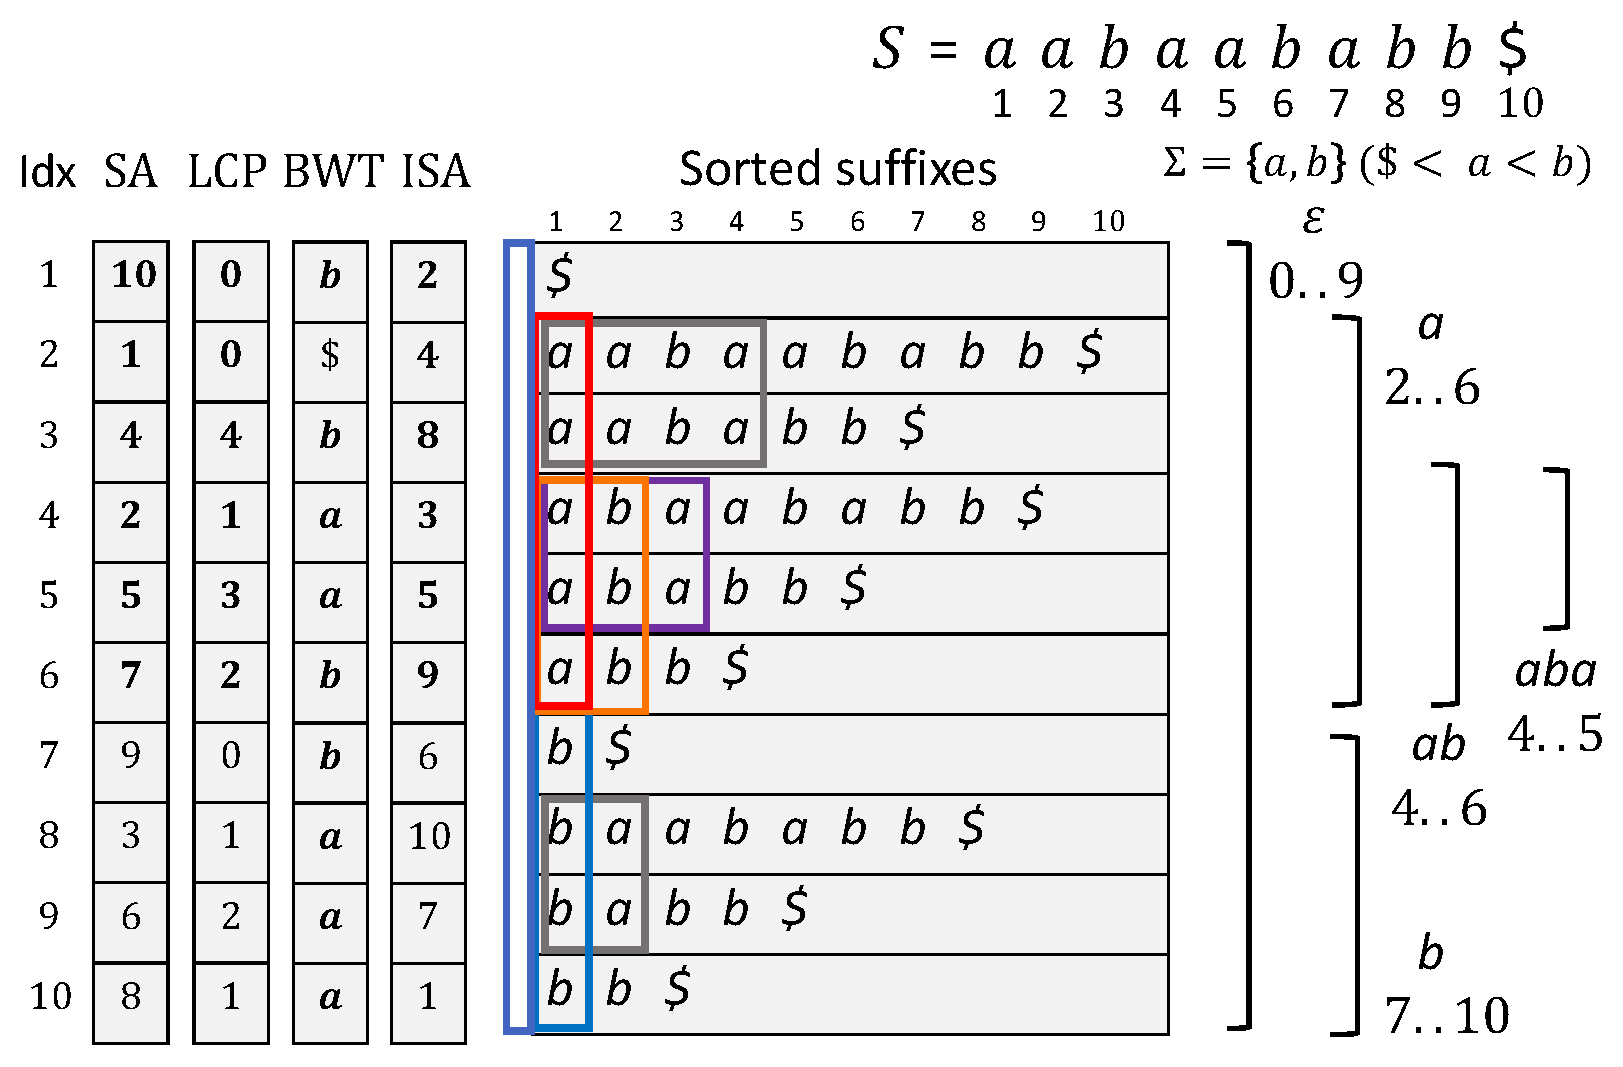
\includegraphics[width=0.70\textwidth]{fig1.pdf}
\vspace{.5\baselineskip}
\caption{An example of indexing arrays of a string $S[1..10] = aabaababb\daller$ of length $n = 10$ over alphabet $\Sigma = \set{a, b}$, whose index starts at $0$, where the left endmarker $S[0]=\#$ and the related suffixes are omitted. 
%%   Inside and to the right of the panel for sorted suffixes, each bold rectangle $R = [i..j]\times [0..\ell-1]$ and square bracket
%% indicate a rich representation $(i..j, \ell)$ of a repeat of $S$ and 
%% the associated SA-interval $i..j$, respectively. 
}\label{fig:example:arrays}
\end{figure}
%%%%%%

%%%% 
\section{Solution}
\label{sec:solution}

In this section, we present an $O(e_{\max})$-expected time solution over an integer alphabet.

\subsection{Outline of the algorithm}
%%%
Let $\Sigma$ be an alphabet with $|\Sigma(S)| \ge 2$ characters. 

\subsubsection{Top-level structure}
%%%% 
In \cref{algo:main}, we show the top-level structure of our algorithm for transforming the suffix array of a string $S$ with auxiliary structures with length $n$ into the CDAWG $G$ of the string. In preprocessing, an index structure $\sig I = (\SA, \ISA, \LCP, S)$ is constructed from an input string~$S$ of length $n$ over $\Sigma$ in linear time using appropriate construction algorithms~\cite{navarro2016cds:book,navarro2021indexing:ii}.
In runtime, the CDAWG $G$ of $S$ is constructed on $\sig I$. 

%%%%
{
% \setlength{\interspacetitleruled}{0pt}%
\setlength{\algotitleheightrule}{0pt}%
\begin{algorithm}[h]
  \caption{Transforming $SA$ and $S$ into its CDAWG $G$.
    %% Transforming the suffix array of a string $S$ with auxiliary structures with length $n$ into the CDAWG $G$ of the string.
  }\label{algo:main}
\KwPreproc{Construct an index $\sig I = (\SA, \ISA, \LCP, S)$ from $SA$ and $S$.}  
\KwRuntime{Perform the following steps}
\Begin{
    Compute $\LPT[+](S) \gets \Rec(\pair{1..n, 0}, \sig I)$\;
    $G \gets$ the DAG obtained from $\LPT[+](S)$ by merging non-maximal nodes to maximal nodes\; \label{line:main:merge}
    Return the CDAWG $G$\; 
}
\end{algorithm}
}
%%%%%%%%%

In an application senario in a human genome repository, the structure $\sig I$ will be constructed once, reside on memory using $O(n)$ space, and be used many times for the generation of the CDAWG in $O(e_{\max})$ time and working space per execution, and other purposes, such as the standard string search.

To describe our algorithm, we will introduce a virtual rooted tree $\LPT[+](S)$, called the \textit{extended longest common prefix tree} of $S$ in the following subsections.
Intuitively, $\LPT[+](S)$ is an edge-compacted rooted tree $T = (\sig V_+, \sig E_+, \eps)$ obtained from the CDAWG $G = (\sig V = \MR(S), \sig E, \eps)$ of $S$, by cutting all non-primary arcs in $\sig E$ to separate them from maximal repeats, and replacing the destinations of arcs with fresh dammy nodes. Its node set is the union $\MR(S)\cup \Delta(S)$ of the set $\MR(S)$ of all maximal repeats and the set $\Delta(S)$ of dammy nodes representing non-maximal repeats. $\LPT[+](S)$ can be stored in $O(e_R)$ words, and can be easily converted into the CDAWG $G$ in $O(e_R)$ time. 

\subsubsection{Recursive subprocedure}
%%%% 
In \cref{algo:rec}, we show the recursive subprocedure $\Rec$ that given the triple $\pair{1..n, 0}$ for the empty string $\eps$, recursively constructs the extended LPT tree $T = \LPT[+](S)$ of a string $S$ on an index structure~$\sig I$. It systematically enumerates the set $\MR(S)$ of all maximal repeats, a class of special factors of $S$, in top-down manner from shorter to longer. In the procedure $\Rec$, each maximal repeat $u$ is encoded as the triple $\pair{i, j, \ell} = \pair{i..j, \ell}$, called the rich-representation, or simply the \textit{triple} of $u$, where $i..j$ is its SA-range of $u$ in $SA$ and $\ell = |u|$ is its length.

The procedure $\Rec$ works as follows: 
%%where maximal repeats are a class of special factors of $S$. 
\begin{itemize}
\item It starts with the triple $\op{rep}(\eps)$ of the shortest maximal repeat, i.e., $\eps$, and the initial DAG $G = (\set{\eps}, \emptyset{}, \eps)$. 
  
\item At each iteration with the triple $\op{rep}(u) = \pair{i..j, \ell}$ of a maximal repeat $u \in \MR(S)$, it generates the triples of a maximal repeat $v_b$ in $\MR(S)\setminus{\eps}$ as a children of $u$ for possible character $b\in\Sigma$, and then, recursively call itself with $v$ and $G$ as arguments. The generation of children of the parent $u$ will be described in the later subsections. 
\end{itemize}

To show the correctness and time complexity, we will show that $\Rec$ simulate a top-down traversal of $\LPT[+](S)$ by visiting all of $O(\mu(S))$ members of $\MR(S)$, following $O(e_R(S))$ arcs, and backtracking when it eventually reaches a non-member of $\MR(S)$.
In the following subsections, we will explain more details of the above procedure. 

%% The tree $\LPT[+](S)$ is rooted at the empty string $\eps$ as the shortest maximal repeat, and whose edge set $\sig E_+ = \sig E \cup \sig F$ consists of the set $\sig E$ of all edges connecting maximal repeats, and additionally contains a set $\sig F$ of edges that are associated with the failure of traversal. 

%%%%%%%%%%%%%5
\begin{algorithm}[t]
  \caption{
    A subprocedure $\Rec$ for constructing the extended LPT-tree $\LPT[+](S)$ of the string $S$ on an index $\sig I = (\SA, \ISA, \LCP, S)$.
    %% for enumerating the set $\MR(S)$ of all maximal reepeats of the string $S$ prefixed by the word $u := \getfactor(i..j, \ell)$. 
}\label{algo:rec}
%%%\medskip
  \KwInput{
    A triple $\pi = \pair{i..j, \ell} \in \RR$ and a rooted tree $T = (\sig V_+(T), \sig E_+(T), \eps)$. 
  }
  \KwOutput{
    A subgraph $T = (\sig V_+(T), \sig E_+(T), \eps)$ of $\LPT[+](S)$. 
  }
  \textbf{procedure} \Rec$(\pi, T)$\;
  \Begin{
      \Comment{Pre-condition: $\pi = \pair{i..j, \ell}$ represents a maximal repeat, say $u$, in $\MR(S)$.}
      %% $Children \gets \emptyset$\; 
      $Children \gets \GenChildren(i..j, \ell, \op{undef})$\Comment*{See \cref{lem:genchildren}}
      \label{line:recmr:for:begin}
      \For {each child $(c, \tau_c = \pair{i_c..j_c, \ell_c})$ in $Children$}{
             \Comment{Post-condition:
               $c \in \RChar(u)$ is a branching character and 
               $\tau_c$ represents
               an $c$-child $\rext{uc} \in \MR(S)$ of $u$. 
             }
             $\sig V(T) \gets \sig V(T) \cup\set{ \tau_c }$
             \Comment*{Adding a node to $\sig V(T) = \MR(S)\cup\Delta(S)$}
             $\sig E(T) \gets \sig E(T) \cup\set{ (\pi, \tau_c) }$
             \Comment*{Adding an arc to $\sig E(T) = \sig E\cup\sig F$}
             \uIf (\comblk{See \cref{lem:leftmaximal:character}}) {$\isLeftBranching(i_c..j_c, \ell_c)$}{
               $\Rec(\tau_c, T)$
               \Comment*{A branching node $\tau_c \in \sig M$ and $(\pi, \tau_c) \in \sig E$, resp.}
               \label{line:recmr:for:end}
             } %% If
             \Else{
               $\rhd$ do not recurse
               \Comment*{A dammy leaf $\tau_c \in \Delta$ and $(\pi, \tau_c) \in \sig F$, resp.}
             } %% Else
       } %% for 
    }
\end{algorithm}
%%%%%%%%%%%%%%%%%

\subsubsection{Constant-size Representation of factors}
%%% 
%% We encode any factor, including maximal repeats, of $S$ in a constant-sized representation as follows so that it can be operated in constant time.
We introduce a representation of any factor of $S$ in constant space so that it can be manupilated in constant time. 
The \textit{rich representation} of a factor $u$ of $S$ is a triple $\tau = (i, j, \ell) \in [n]^3$, where
\begin{itemize}
\item the pair $(i, j)$ with $1\le i\le j\le n$ represents the \textit{SA-range} $i..j\subseteq 1..n$ of $u$ that is the maximal range w.r.t.~set-inclusion consisting of all suffixes of $S$ prefixed by $u$, and  
  
\item the integer $\ell\ge 0$ represents the length of the factor $u$, namely, $\ell = |u|$. 
\end{itemize}

We denote by $\RR$ the set of the rich-representation of all factors of $S$.

\subsection{Enumeraton of maximal repeats of $S$}  
%%\subsection{The $\LPT[+](S)$ tree}
%%% 
The tentative goal here is to generate all maximal repeats without duplicates in amortized constant time per solusion. For the purpose, we introduce the LPT tree of $S$, $\LPT[+](S)$, which will be shown to be a subgraph of the suffix tree of $S$ later. Then, we give a high-level description of our algorithm.

\subsubsection{Relationship between $\Stree(S)$ and $\CDAWG(S)$}
%%%
Consider the suffix tree $\Stree(S) = (V, E, \underline\eps)$ of a string $S$. 
%% Recall that $\underline u$ is the locus of a factor $u$ such that $\str(\underline u) = u$. 
In $\Stree(S)$, we observe that all branching nodes correspond the loci $\underline u$ of all right-branching factors $u$ of $S$, while all leaves correspond to the loci $\underline s$ of all suffixes $s$ of $S$.

\begin{remark}\label{remark:one:primary}
  For any factor $u \in \Sigma^*$ of $S$, the conditions (1)--(3) are equivalent:
  \begin{enumerate}[(1)]
  \item The locus $\underline{u}$ of $u$ in the CDAWG of $S$ is a branching node and $u$ is the string label of the longest path from the source to $\underline{u}$. 
  \item The locus $\underline{u}$ of $u$ in the suffix tree of $S$ is a branching node and has two or more incoming suffix links. 
  \item The string label $u$ is a maximal repeat of $S$, i.e., $u \in \MR(S)$. 
  \end{enumerate}
\end{remark}

We need a few technical definitions. 
For any factor $u \in \Sub(S)$, we define the right-closure of $u$, denoted $\rext{u}$, to be the string obtained from $u$ by maximally extending $u$ rightwards while the occurrence of the resulting substring does not change, i.e., $\Spos(\rext{u}) = \Spos(u)$ holds.
Similarly, we can define the left-closure of $u$, denoted $\lext{u}$ by symmetry. 
%%
For example, consider a string  $S[1..n] = \mathtt{aabaababb\$}$ of length $10$. For a factor $aa$ with $\Spos(aa) = \set{1, 4}$, its right-closure is $\rext{aa} = aaba$. On the other hand, for a factor $a$ with $\Spos(a) = \set{1,2,4,5,7}$, its right-closure is $\rext{a} = a$. 

%% %%This definition is well-defined since the longest path is closed under prefix.
%% Next, in the suffix tree $T$ of $S$, with a slight abuse of terminology, a (unique) path $\pi$ from the root to a node $\underline v$ is said to be \textit{primary} if its corresponding path in $G$ is primary. Again, a primary path is closed under prefix. Then, any arc $f = (\underline u, \underline v)$ in $T$ is said to be \textit{primary} if it is included in a primary path $\pi$ to $\underline v$, and \textit{non-primary} otherwise. 

%% From the equivalence shown in \cref{remark:one:primary}, we introduce the primary arcs in the CDAWG $G$ and suffix tree $T$ of $S$. In $G = \CDAWG(S)$,  any arc $f = (\underline u, \underline v)$ is said to be \textit{primary} if it is included in the longest path from the root to node $\underline v$, and \textit{non-primary} (or secondary) otherwise.
%% %%This definition is well-defined since the longest path is closed under prefix.
%% Next, in the suffix tree $T$ of $S$, with a slight abuse of terminology, a (unique) path $\pi$ from the root to a node $\underline v$ is said to be \textit{primary} if its corresponding path in $G$ is primary. Again, a primary path is closed under prefix. Then, any arc $f = (\underline u, \underline v)$ in $T$ is said to be \textit{primary} if it is included in a primary path $\pi$ to $\underline v$, and \textit{non-primary} otherwise. 

\subsubsection{The extended longest common prefix tree of $S$}
%%%
We introduce subgraphs $\LPT(S)$ and $\LPT[+](S)$ of $\Stree(S)$ in the followings. First, we define the subsets of nodes $\sig V(S), \Delta(S) \subseteq V$ and the subsets  of arcs $\sig E(S), \Delta(S)\subseteq E$ as follows: 
\begin{itemize}
\item $\sig V$ is the subset of the nodes corresponding to all maximal repeats, that is, $\sig V = \set{ \underline u \mid u \in \MR(S) }$. 
  
\item $\sig E \subseteq E$ is the subset of all arcs $f = (u, v)$ in $E$ that connect maximal repeats in $\MR(S)$, that is, $\sig E = \sete{ (\underline u, \underline v) \in E \mid \set{u, v} \subseteq \MR(S) }$.

\item $\sig F\subseteq E$ is the subset of all arcs $f = (u, v)$ in $E$ that connect a maximal repeat $u$ and a non-maximal repeat $v$, that is, $\sig F = \sete{ (\underline u, \underline v) \in E \mid u \in \MR(S), v \not\in \MR(S) }$.  
%% $\sig E_+(S) = \sig E(S) \cup \sig F(S)$ is the subset of $E$, where
  
\item $\Delta(S) = \set{ \underline v \mid f = (\underline u, \underline v) \in \sig F }$ is the set of the destinations of all arcs in $\sig F$.
%% $\sig V_+(S) = \sig V(S) \cup \Delta(S)$ is the subset of $V$, where 
\end{itemize}

By construction,
%% it follows that $\sig V(S)\subseteq \sig V_+(S) \subseteq V(S)$ and $\sig E(S)\subseteq \sig E_+(S) \subseteq E(S)$. Moreover,
$\sig V_+(S)$ contains the shortest maximal repeat $\eps$. The DAG $\LPT(S)$ is called the longest common prefix tree of $S$ in the literature.  

\begin{definition}[Belazzougui \textit{et al.}~\cite{belazzougui:nunial:gagie:prezza:raffinot2015composite}, Inenaga \textit{et al.}~\cite{inenaga:iwoca2024computing:maw}]
  We define the extended longest common prefix tree of $S$ to be the rooted DAG $\LPT[+](S) = (\sig V_+(S), \sig E_+(S), \eps)$, where 
  $\sig V_+(S) = \sig V(S) \cup \Delta(S) \subseteq V$ is the node set, $\sig E_+(S) = \sig E(S) \cup \sig F(S) \subseteq E$ is the arc set, and $\eps \in \sig V_+(S)$ is the root. 
\end{definition}

Blumer \textit{et al.}~\cite{blumer1987complete} showed the properties of the CDAWG $G$ of $S$, which is the minimum state DFA of $\Suf(S)$ with path-compression. We define the \textit{end-equivalence relation} $\equiv_{epos}$ over $\Sub(S)$ by $x \equiv_{epos} y \iff\Epos(x) = \Epos(y)$.
%%%
Each node $\underline u$ of $G$ with $u \in \Sub(S)$ represents an equivalence class, denoted by $[\rext{u}]^S_{epos} \subseteq \Sub(S)$, of factors of $S$ with respect to $\equiv^S_{epos}$. That is, $\underline u := [\rext{u}]^S_{epos} = \sete{ v \in \Sub(S) \mid u \equiv_{epos} v}$.
%% Then, each node $\underline u$ of $G$ represents the equivalence class $[\rext{u}]^S_{epos} \subseteq \Sub(S)$ of factors of $S$ with a representative $u \in \Sub(S)$ w.r.t.~$\equiv^S_{epos}$, namely, $\underline u := [\rext{u}]^S_{epos} = \sete{ v \in \Sub(S) \mid u \equiv_{epos} v}$.
%%%
%% Usually, the longest element, denoted by $\Value(\underline u)$ is used as the representative of $\underline u = [\rext{u}]^S_{epos}$.
The representative of $\underline u = [\rext{u}]^S_{epos}$ is the longest element, which we denote by $\Value(\underline u)$. 
Each member $v$ of the equivalence class $[\rext{u}]^S_{epos}$ is the string label of a path from the root to node $\underline u$. 
All arcs in the CDAWG $G$ can be classified as either primary or non-primary. An arc $f = (\underline u, \underline v)$ is said to be \textit{primary} if it is included in the longest path from the root to node $\underline v$, and \textit{non-primary} (or secondary) otherwise.
Note that only a subset of arcs of $\Stree(S)$ can be included in $\CDAWG(S)$ in general. 

\begin{lemma}[Belazzougui \textit{et al.}~\cite{belazzougui:nunial:gagie:prezza:raffinot2015composite}]\label{lem:lpt:edge:classification}
  The arc subsets $\sig E$ and $\sig F$ of $\LPT[+]$ correspond to the sets of all primary arcs and all non-primary arcs in $G = \CDAWG(S)$. That is, for all pair of factors $u, v\in \Sub(S)$, the arc $f = (\underline u, \underline v)$ in $\sig E_+$ and the corresponding arc $f' = ([\rext{u}]^S_L, [\rext{v}]^S_L)$ satisfies the conditions (1) and (2) below: 
\begin{enumerate}[(1)]  
\item $f \in \sig E\cup \sig F$ if and only if $f$ is an arc of $G$. 
\item Moreover, (i) $f \in \sig E$ if and only if $f'$ is a primary arc of $G$, while (ii) $f \in \sig F$ if and only if $f'$ is a non-primary arc of $G$.
\end{enumerate}
\end{lemma}

\begin{proof} TBD. 
\end{proof}

From \cref{lem:lpt:edge:classification}, we refer to the arcs $f$ of $\LPT[+](S)$ as \textit{primary} if $f \in \sig E$ and as \textit{non-primary} if $f \in \sig F$ without confusion. Then, we can identify $\LPT[+](S)$ and $G = \CDAWG(S)$, where we can obtain the former from the latter by replacing each secondary arc $f = (\underline u, \underline v)$ by a new arc $f' = (\underline u, \underline {v_f})$ with a new end point $\underline{v_f}$ and the associated string label $v_f = \Value(\underline u)\cdot \lab(f) \in \Sigma^+$. 

\subsubsection{Simulating a traversal of $\LPT[+](S)$}
%%%%
Since the node set of $\LPT[+](S)$ equals the set $\MR(S)$ as its nodes, we can enumerate all maximal repeats in $\MR(S)$ by a top-down traversal of $\LPT[+](S)$ using backtracking starting from the representation $\tau_\eps \in \RR$ for the root $\eps$, and expanding the current representation $\tau \in \RR$ for a maximal repeat $u \in \MR(S)$ into the set of its children $Children(\tau) \subseteq \RR$.
Below, we will inductively construct a spanning tree over the set $\MR(S)$ by induction on the length of a string as follows.

In the base case, we can easily see that the empty string $\eps$ is the shortest member of $\MR(S)$ due to the assumption $|\Sigma|\ge 2$. Then, it is easy to see that the triple for $\eps$ is given by $\pair{1..n, 0}$. 

In the induction case, we try to generate the triple for a maximal repeat $v\in \MR(S)$ from the triple for a shorter maximal repeat $u\in \MR(S)$.
%% Then, the parent $u$ of a maximal repeat $v \in \MR(S)$ is the maximal repeat $u \in \MR(S)$ such that
For any arc $f = (\underline u, \underline v) \in \E\cup\F$ in $\LPT[+](S)$, we say that $u$ is the \textit{parent} of $v$, and $v$ is a \textit{child} of $u$. 
Generation of the set $Children(\tau)$ can be done as follows.

%% Note that a factor $v$ of $S$ is left-branching only if its SA-range $i..j$ have width two or more, i.e., $|i..j| \ge 2$. 

\begin{lemma}\label{lem:maxrep:howto:child}
  Let $\LPT[+](S) = (\sig V_+, \sig E_+, \eps)$
  For any maximal repeat $u \in \Sigma^*$ in $\MR(S)$ and any non-empty string $v \in \Sigma^+$, the following conditions (1) and (2) are equivalent: 
\begin{enumerate*}[(1)]
\item $v \in \sig V_+$ and $u$ is the parent of $v$;  
\item
  \begin{enumerate*}[(i)]
  \item $v = \rext{(ua)}$ for a character $a\in \Sigma$, and 
  \item $v$ is a left-branching factor of $S$. 
    %% \item $|i..j| \ge 2$ with
    %% the SA-range $i..j$ of $v$. 
  \end{enumerate*}
\end{enumerate*}
\end{lemma}

{
%% \setlength{\interspacetitleruled}{0pt}%
\setlength{\algotitleheightrule}{0pt}%
\begin{algorithm}[h]
  \caption{
    \textbf{Procedure} $\GenChildren(\pair{i..j, \ell_*}, Children)$.  
  }\label{algo:genchildren}
  %% \KwInput{the triple $W = (i..j, \ell_*)$ for a factor of $S$.}
  %% \textbf{Procedure} $\GenChildren(\pair{i..j, \ell_*}, Children)$:\\
  \Comment{\textit{Notes}: $S$ and $SA$ at \cref{line:genchildren:compute:ch} are only for explanation, and can be omitted.
  }
  %% \Begin{
      \If  (\comblk{
        $|i..j| = j - i + 1$.
        %% $\pair{i..j, \ell}$ has no unique occurrences
      })
           {$|i..j| \ge 2$}
           %% {$j - i + 1 \ge 2$}
      {
        $(m, \ell_m) \gets RMQ_{LCP}(i+1, j)$
        \Comment*{$\ell_m = LCP[m]$}
        \uIf (\comblk{$i..j$ is monotone}) {$\ell_* < \ell_m$}{
          %% $p \gets SA[i]$\;
          $ch \gets S[SA[i]+\ell_*]$
          \Comment*{Notes: $ch$ is used for explanation only}
          \label{line:genchildren:compute:ch}
          $Children.\append(\pair{ch, \pair{i..j, \ell_m}})$
          \Comment*{A child $\pair{ch, \pair{i..j, \ell_m}}$}
        }
        \Else  (\CM{$\ell_* = \ell_m$} and $[i,j]$ is diverse) 
        {
          $\GenChildren(\pair{i..m-1, \ell_*}, Children)$\; 
          $\GenChildren(\pair{m..j, \ell_*}, Children)$\;
        }
      }
      \Return $Children$\;
  %% } %% Begin
\end{algorithm}
}
%%%%%%%%%%%%%%%%%

\subsection{Generation of the set of child triples}
%%%% 
An SA-range $i..j$ is called an \textit{$\ell$-range} if the lcp of all suffixes starting  with positions in $SAi..j$ equals~$\ell$, i.e.,
\begin{align}
  \ell
  &= lcp(\set{ S[p..n] \mid p = SA[k], k \in i..j } ) 
\\&= \min\sete{ LCP[k] \mid k \in [L+1..R] },   
\end{align}
where $LCP[k] = lcp(S[p..n], SA[q..n]])$ with $p = SA[k]$ and $q = SA[k-1]$. 
Then, an index $k \in i+1..j$ such that $LCP[k] = \ell$ is called a \textit{$\ell$-index}. 
Cosider the suffix tree $\sig T$ of a string $S$.
%% We say that a triple $\tau = (i..j, \ell)$ is a child of triple $\tau_0 = ([L_0..R_0], \ell_0)$
For two triples $\tau_i$ for factors $u_i$ for every $i = 1,2$, we say that $\tau_1$ is the parent (resp.~a child) of $\tau_2$ if and only if $u_1$ is the parent (resp.~a child) of $u_2$.

We remark that any SA-range $i..j$ without a length component $\ell$ implicitly represents a right-maximal factor of $S$. More precisely, we observe that a triple $\pi = \pair{i..j, \ell}$ represents a right-maximal factor of $S$ if and only if $i..j$ is an $\ell$-range. We always assume that a parent $\pi$ satisfies this condition. 
For generating the set $Children(\tau)$ of all child triples of a given parent tripel $\tau$, we use the following lemma, shown by . Abouelhoda, Kurtz, and Ohlebusch~\cite{abouelhoda2004replacing}. 

\begin{lemma}[Abouelhoda \textit{et al.}~\cite{abouelhoda2004replacing}]\label{lem:child:ranges}
  Let $\pi = [i_0..j_0]$ be any $\ell$-range.
  If $m_1 < m_2 < \dots < m_k$ are the $\ell$-indexes in ascending order, then the child ranges of $\pi$ are
  $[i_0..m_1-1], 
   [m_1..m_2-1], 
   \ldots,
   [m_k..j_0]$.  
\end{lemma}

Abouelhoda \textit{et al.}~\cite{abouelhoda2004replacing} presented an algorithm for generating all child triples using an extra array $\op{childtab}[1..n]$ of cells with three integer fields $\op{up}, \op{down}$, $\op{nextIndex} \in [n]$ in addition to $\SA$ and $\LCP$. 
%%However, the method is not suitable to our purpose. 
%%% 
Instead of the $\op{childtab}$ array, we present another method using $\SA$ and the RMQ structure on $\LCP$ (denoted $RMQ_{\LCP}$) as follows.%
%%%% 
\myfootnote{We remark that the string $S$ in $\GenChildren$ can be omitted since it is used to get right-brancing characters, only for explanation, and not used by $\Rec$ of \cref{algo:rec}. }
%%%% 
%% generate the set $Children(\pi)$ of all child triples of a parent triple $\pi$. 
As a key component,
we use the implementation of the colored range query
based on \cref{lem:child:ranges}, proposeby Muthukrishnan~\cite{muthukrishnan2002efficient} (see also the textbook by Ohlebusch~\cite{ohlebusch2013bookbioinfo}).

\begin{lemma}[Muthukrishnan~\cite{muthukrishnan2002efficient} and Ohlebusch~\cite{ohlebusch2013bookbioinfo}]\label{lem:genchildren}
  The set of all child ranges of an $\ell$-range $i..j$ can be enumerated in $O(occ)$ time in $O(\sigma)$ working space
  using the $RMQ_{LCP}$ structure of $O(n)$ words, 
where $occ$ is the number of the child renges to output.  
\end{lemma}

Based on \cref{lem:genchildren}, \cref{algo:genchildren} presents the procedure $\GenChildren$, which recusively generates the set of child triples
\begin{align}
  Children(\pi)
  &= \sete{ (c, \tau_c) \mid c \in \LChar(u), \tau_c = \pair{i..j, \ell} \in Children(\pi)}, 
\end{align}
invoked with a parent triple $\pi = \pair{i..j, \ell_*}$ with $\ell_*$-range for a maximal repeat $u$ and the pointer $Children$ to the empty set $\emptyset$,
where $\tau_c$ is the triple for a maximal repeat $\rext{(uc)}$ with a branching character $c \in \LChar(u)$.

\subsection{Efficient test of the left-brancing condition}
%%% 

Recall that a repeat is maximal if and only if it is both left- and right-maximal in $S$. Since the node set $\sig V+$ of $\LPT[+](S)$ is closed under taking parents, we have the next lemma.

\begin{lemma}\label{lem:prune:leftbranch}
Suppose that a triple $\pi$ is an ancestor of a triple $\tau$. If the substring $ub$ defined by $\tau$ is left-branching, the substring $u$ defined by $\pi$ is also left-branching. 
\end{lemma}

\begin{proof}
  For any $v = ub$ with some $b \in \Sigma$, we can show that
  $\LChar(ub) \subseteq \LChar(u)$, and thus that $|\LChar(ub)| \le |\LChar(u)|$. On the other hand $ub$ is right-brancing in $S$ if and only if $2\le |\LChar(ub)|$. It immediately follows that $2 \le |\LChar(u)|$ meaning that $u$ is right-brancing in $S$. This shows the lemma. 
\end{proof}


Since the nodes of the set $\sig V_+$ represents all and only the right-branching factors, \cref{lem:prune:leftbranch} implies the next rule.

\begin{itemize}\item[]
\quad\textsc{Pruning rule}: {Every non-left-branching triple is pruned.}
\end{itemize}

We explain how to efficiently test whether a given triple $\tau = \pair{i..j, \ell}$ represents a left-branching factor of $S$. For this purpose, we use the following lemma, which is a slight modification of Narisawa \textit{et al.}~\cite[Lemma~10]{narisawa2007efficient}.

\begin{minipage}{\textwidth}
\begin{lemmarep}[Narisawa \textit{et al.}~\cite{narisawa2007efficient}]\label{lem:leftmaximal:character}
  For the triple $\tau = (i..j, \ell)$ for any substring~$u$ of $S$,
  \begin{enumerate}[(1)]
\item $u$ is not left-branching in $S$ if and only if  
\item (i) $S[p-1] = S[q-1]$ and (ii) $j - i = \id{ISA}[p-1] - \id{ISA}[q-1]$, 
\end{enumerate}
where $p = SA[i]$ and $q = SA[j]$.
\end{lemmarep}
\end{minipage}
\medskip 

\begin{proof}
%%We add clause (*)  
We let $p = SA[i], q = SA[j]$. 
$(1)\Implies (2)$: Suppose that $u$ is not left-branching in $S$.
Then, all occurrences of $u$ in $S$ have the same previous characters $c \in \Sigma$ in $\Spos(u)$. Thus, it immediately follows that $BWT[i..j]$ is monotone.
Let $\varphi: k \mapsto ISA[SA[k]-1]$. By observing $\varphi$ coincodes to the LF-mapping~\cite{Ferragina05:FM}, claim (2) immediately follows. 
%%% 
$(2) \Implies (1)$: 
Suppose (2), and to contradict that $\neg$(2) $u$ is left-branching in $S$. Let $I = i..j$. Then, there exist a pair of preceding characters $c = S[p-1], d=S[q-1]$ with $c\not= d$ for some $p, q \in \Spos(u)$. It follows that $\varphi$ transforms the positions in  $SA[i..j]$ into at least two, mutually disjoint, non-empty ranges $I_c, I_d$ with $I_c\uplus I_d = I$ starting with $c$ and $d$, respectively. By assumption (2.i), we see that positions $SA[i]$ and $SA[j]$ move into the same range, say $I_c$ with $i_c := \varphi(i)$ and $j_c := \varphi(j)$ as the left and right ends of $I_c$ since $\varphi$ preserves $<_\lex$. 
Since both of $I_c$ and $I_d$ are non-empty, we have $j_c - i_c + 1 = |I_c| < |I| = j - i + 1$; contradiction to assumption (2.ii). By contradiction, we conclude condition (1) holds. 
%% \qed   
\end{proof}

From \cref{lem:leftmaximal:character}, we can implement the procedure $\isLeftBranching(i..j, \ell)$ for testing the left-branching property of a triple $\tau = \pair{i..j, \ell}$. The code for $\isLeftBranching$ is omitted. 


%%%%%%%%%%%%%%%%%%%%%%%%%%%%%%%%%

%% \subsubsection{Computing a set of right-branching characters}
%% %%% 
%% In \cref{algo:genchildren}, we show a procedure $\GenChildren$ for computing the set of all child ranges of an $\ell$-range, based on precomputed arrays $\LCP, \SA, S$.


%% At the top-level, the procedure is invoked with the triple $\pi = (i..j, \ell_*)$ for a factor of $S$ and the pointer to the set $Children = \emptyset$. At every iteration of $\GenChildren[]$, the following pre-condition must be ensured: $\ell_*$ is the lcp-length of all suffixes in the range $i..j$, namely, $RMQ_{LCP}(i+1, j) = \ell_*$ must hold.

%%       %% \If{ $Children = \op{undef}$ }{
%%       %%   We let $Children$ to be the pointer to a newly created set $\emptyset$. 
%%       %% }



%% \begin{toappendix}
%% By definition, we see that
%% $(i,j,\ell) \in \RR$ if and only if
%% \begin{enumerate*}[(i)]
%% \item $k \in i..j \iff u = S[p..p+\ell-1]$ for all $k$, and
%% \item $\ell = minLCP(i,j)$,
%% \end{enumerate*}
%% where $p = SA[k]$ and $minLCP(i,j)$ denotes the minimum LCP-values of an SA-range $i..j$ defined to be $minLCP(i,j) := \max_{i\le k\le j} lcp(S[p..n])$.

%% \begin{remark}[SA-ranges as a representation of right-maximal factors]
%%   We remark that any SA-range $i..j$ without a length component $\ell$ implicitly represents a right-maximal factor of $S$ as follows. By letting $\ell$ to be the min-lcp value of the range, that is, $\ell := minLCP(i,j)$, we obtain the triple $(i..j, \ell)$ representing a $u = S[p..p+\ell-1]$ of $S$, where $p = SA[k]$ with an arbitrary $k \in i..j$. Then, it is not hard to see that $u$ is rigit-maximal in $S$.
%% \end{remark}
%% \end{toappendix}

\subsection{Merging dammy leaves to branching nodes (TBD)}
%%%
(This subsection is incomplete, and the complexity of merging is  still open.)

At \cref{line:main:merge} in \cref{algo:main}, we merge all dammy leaves in $\Delta(S)$ for non-maximal factors into the associated equivalence classes of branching nodes in $\sig V$.

Consider the extended LPT tree of $S$, $\LPT[+](S) = (\sig V_+(S), \sig E_+(S), \eps)$. We introduce the set $\sig W(S)$ of Weiner-links as follows. 
For any node $\underline u \in \sig V_+(S)$ with string labels $u$, and any character $a \in \Sigma$, if $v = au$ is a factor of $S$, $au \in \Sub(S)$, we put the (either soft or hard) Weiner link $g = (\underline u, \underline v)$ from $\underline u$ to the locus $\underline v$ of $v$ with character label $\lab(g) = a$ in $\LPT[+](S)$. Then, we say that $u$ is the parent of $v$, and $v$ is a child of $u$ w.r.t.~$\sig W(S)$. 
Moreover, the link $g$ is \textit{hard} if $\underline v$ is a real (right branching) node, and \textit{soft} otherwise (that is, $\underline v$ is a locus on an arc).
%% 
We can easily show that the total number of hard and soft Weiner links are upperbounded by the number $e_L$ of left-extensions of maximal repeats of $S$. 

Without loss of generality, we identify the triples and the nodes of $\LPT[+](S)$. Based on the above definition of $\sig W(S)$ and its parent-child relation, we show the next lemma, which is the dual of \cref{lem:prune:leftbranch}. 

\begin{lemma}\label{lem:prune:rightbranch}
Suppose that a triple $\pi$ is the parent of a triple $\tau$ with respect to the Weiner links in $\sig W(S)$. If the substring $au$ defined by $\tau$ is right-branching, the substring $u$ defined by $\pi$ is also right-branching. 
\end{lemma}

\begin{proof}
  By symmetry, the lemma follows from the proof of \cref{lem:prune:leftbranch}. 
  %% If $v = au$ for some $a \in \Sigma$, we can easily show that
  %% $\RChar(au) \subseteq \RChar(u)$, and thus that $|\RChar(au)| \le |\RChar(u)|$. On the other hand $au$ is right-brancing in $S$ if and only if $2\le |\RChar(au)|$. It immediately follows that $2 \le |\RChar(u)|$ meaning that $u$ is right-brancing in $S$. This shows the lemma. 
\end{proof}

Recall that $\sig V$ is the set of nodes for all maximal repeats in $\MR(S)$ and $\eps \in \sig V$. 
We let $\sig W$ to be the set of all Weiner links $g = (\underline u, \underline{au})$ that connect elements of $\sig V$ with a character $a \in \Sigma$, that is, $\set{u, au} \subseteq \MR(S)$.

Now, we define the \textit{Weiner-link counterpart} of $\LPT[+](S)$, denoted by $\LPT[-](S) = (\sig V_-, \sig W_-, \eps)$ as follows.
\begin{itemize}
\item $\sig F_- = \sete{ g = (\underline u, \underline au) \mid u\in\MR(S), u\not\in \MR(S) }$ is the set of all Weiner links $g = (\underline u, \underline au)$ that connect maximal nodes of $\sig V$ to non-maximal nodes. 
  %%, that is, $u\in\MR(S)$ and $u\not\in \MR(S)$.
\item Let $\sig V_- = \sig V \cup \Delta_-$, 
  where $\Delta_- = \sete{\underline{au} \not\in\sig V \mid g = (\underline u, \underline{au}) \in \sig F_-}$ be the set of non-maximal nodes reachable from $\sig V$ by arcs of $\sig F_-$.
  
\item $\sig W_+$ be the union of $\sig W$ and $\sig F_-$. 
\end{itemize}

Then, the extend LPT tree w.r.t.~Weiner links in $\sig W$ is the rooted tree $\LPT[-](S) = (\sig V_-, \sig W_-, \eps)$. 



\subsection{Putting it all together}
%%%

Suppose that an index $\sig I = (\SA, \ISA, \LCP, S)$ is preprocessed from $SA$ and $S$ in \cref{algo:main}. 
Consider the recursive procedure $\Rec$ in \cref{algo:rec}, which is equipped with subprocedure $\GenChildren$ in \cref{algo:genchildren} and the procedure $\isLeftBranching(i..j, \ell)$ in \cref{lem:leftmaximal:character}. 

\begin{trivlist}\item[]
\textit{Proof for \cref{thm:main:cdawg:sa:lcp}}. 
By the construction of $\LPT[+](S)$ and from
\cref{lem:maxrep:howto:child},
\cref{lem:genchildren},
\cref{lem:leftmaximal:character},
the recursive procedure $\Rec$ in \cref{algo:rec} correctly visits all nodes of $\LPT[+](S)$ corresponding to all maximal repeats following all arcs in $\E(S)$ using a depth-first traversal of $\LPT[+](S)$.
From \cref{lem:prune:leftbranch}, we see that if it eventually reaches a non-maximal node in $\Delta(S)$, it correctly stops the search and backtracks. Each arc is added to the arc set whenever it is traversed. Since each node $\underline v$ in $\E(S)\cup \F(S)$ can be reached through exactly one incoming arc, the procedure correctly find all arcs.

At \cref{line:main:merge} in \cref{algo:main}, we can merge 
\qed
\end{trivlist}

%% \subsection{$O(e_{\max})$-worst-case time solution over a constant alphabet}

\bigskip

\subsection{Execution example}

In \cref{fig:run:example}, we show an example run of Algorithm $\MREnum$ for a string $S[0..10] = \mathtt{\#aabaababb\$}$. The black and red trees, respectively, indicate the suffix and the Weiner trees of $S$. Each circle indicates a node with the string label and the triple. A gray node corresponds a maximal repeat. 
We observe that the algorithm $\Rec$ only traverses the suffix tree starting from the root, and enumerates all maximal repeats, by visiting all and only the gray nodes. 

%%%%%%
\begin{figure}[t]
  \centering
  \rule{0.09\textwidth}{0em}
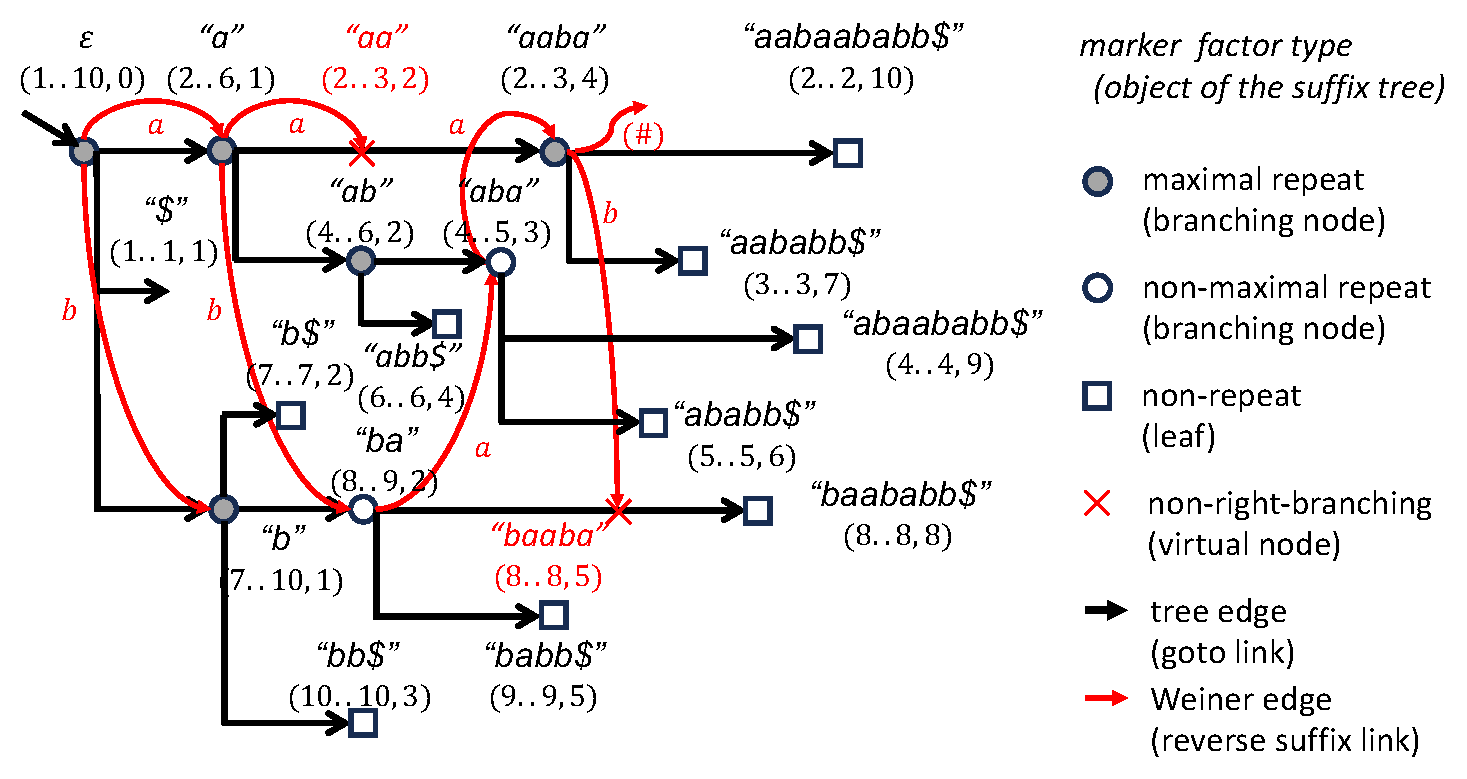
\includegraphics[width=0.7\textwidth]{fig2.pdf}
\vspace{.75\baselineskip}
\caption{An example run of Algorithm $\Rec$ for a string $S = \mathtt{aabaababb\$}$, where the left endmarker $S[0]=\#$ and the related suffixes are omitted. 
}\label{fig:run:example}
\end{figure}
%%%%%%

\subsection{Notes} In the end of this article, we show how to replace these structure of $O(n)$ space with index structures of $o(n)$ space for highly-repetitive strings, such as run-length compressed suffix trees or r-index (Gagie, Navarro, and Prezza~\cite{gagie:navarro:prezza2020fully}), by allowing poly-logarithmic slowdown. Since such repetition-aware string indexes have been widely used as the de facto standard method for storing and searching human genome sequences, the proposed method will largely increase the utility of such sequence indexing structures.

\section{Related work}
%%% 
It is well-known that the problem of transforming the suffix array of a string $S$ into its suffix tree $T$ can be solved in $O(n)$ time and space. This is achieved using the suffix array (SA) and the longest common prefix array (LCP)  with an auxiliary stack of size $\idrm{height}(T)$.
This transformation can be performed by simulating either
a bottom-up traversal of the suffix tree, as shown by Kasai \textit{et al.}~\cite{kasai:lee2001lcp:linear} and Crochemore \textit{et al.}~\cite{crochemore2021book125problems:chap:satostree}, or
a top-down traversal as demonstrated by Abouelhoda, Kurtz, and Ohlebusch~\cite{abouelhoda2004replacing}.

Besides this, most closely related work is recent development of $O(n)$-time transformation algorithms for enumeration of \textit{maximal repeats} of a string $S$ using the \textit{Burrows-Wheeler transform} (BWT), 
%%augmented with the \textit{Wavelet tree}.
which simulate a top-down traversal of the tree of the reversed suffix links, called the \textit{Weiner tree}~\cite{beller:berger2012space:efficient:bbo,nishimoto:cpm2021enum}. 
Since the set of maximal repeats corresponds the node set of the CDAWG of the string, they can be expected to be used as a building block to solve the CDAWG construction problem, too. The latest of them, proposed by Nishimoto and Tabei~\cite{nishimoto:cpm2021enum}, runs in $\Theta(n)$-time and $O(r\,\idrm{polylog}(n))$-space based on the r-index~\cite{gagie:navarro:prezza2020fully}.  

Recently, Cleary and Dood~\cite{cleary2023constructing} proposed an algorithm for constructing the CDAWG of a string in the form of a grammar using the SA-intervals of maximal repeats of the string. However, they did not mention how to compute such SA-intervals in $O(e_{\max})$ time and space. 

In summary, to the best of our knowledge, however, it remains an open question whether the CDAWG can be computed from the SA and LCP arrays in output-sensitive manner.
Specifically, it is not known if this can be done using $O(e_{\max})$ or less time and working space --- in addition to the $O(n)$-size read-only inputs --- for repetitive string with right-extension parameter $e_{\max} \le n$.
On the other hand, the proposed algorithm in this paper shows that it is possible to perform translation from the SA and LCP arrays into the CDAWG in output-sensitive time and space by a novel combination of known techniques.  

%%%% 
\section{Notes}
\label{sec:notes}

The relationship between the size of the CDAWG and the parameter $e_{\max}$ was studied by Raffinot~\cite{raffinot2001maximal}, and the use of $e_{\max}$ as a compression parameter was proposed by Belazzougui \textit{et al.}~\cite{belazzougui:nunial:gagie:prezza:raffinot2015composite}.

%%%% 
\section{Conclusion}
\label{sec:concl}
We presented an output-sensitive algorithm for transforming the suffix array of a string with auxiliary structures of $O(n)$ size into the CDAWG of the same string. 
In conclusion, the combination of the simplicity and efficiency would be practical advantages of our algorithm especially when we deal with collections of highly-repetitive strings in the realworld, e.g., human genome sequences and versioned texts of Wikipedia. 


%%%% end of body %%%%%%%%%%%%%%%%%%

% ---- Bibliography ----
\newpage
\bibliographystyle{plain}
\bibliography{ref}
%% \bibliography{bib/ref,ref}
\end{document}

